\section{Experiments}
\label{sec:experiments}

In order to evaluate the MF model, we perform several experiments using three different datasets. We start by experimenting on the normalization parameters in order to study their impact on the effectiveness of the approach. We then compare the MF ranking functions against other traditional ones. We finally discuss the consequence of \textbf{not} considering the attribute label as a source of potential relevant terms and demonstrate the effectiveness of the proposed weights.

While there are other ways to perform entity ranking on the Web of Data, e.g., one can look at the other SemSearch 2011\footnote{SemSearch2011: \url{http://km.aifb.kit.edu/ws/semsearch11}} candidates, in this evaluation we concentrate on demonstrating how the MF model specifically extends and improves the very popular PRF and DFR frameworks.

\subsection{Datasets}
\label{sec:datasets}

The datasets we are using in our experiments are the following:
\begin{description}
  \item[INEX09] a dataset of 2,491,134 triples from DBpedia containing the description of entities in English, and converted for the INEX evaluation framework~\cite{Perez-Aguera:2010:UBS};
  \item[SS10] the ``Billion Triple Challenge''\footnote{Billion Triple Challenge: \url{http://vmlion25.deri.ie}} (BTC) dataset, containing more than one billion triples, with the assessments of the SemSearch2010\footnote{SemSearch2010: \url{http://km.aifb.kit.edu/ws/semsearch10}} challenge;
  \item[SS11] the BTC dataset with the assessments of the ``Entity Search track'' of the SemSearch2011\footnote{SemSearch2011: \url{http://km.aifb.kit.edu/ws/semsearch11/}} challenge.
\end{description}
The INEX09 dataset is significantly different than the other two based on BTC. Indeed, BTC is a heterogeneous dataset, created from web crawls of several search engines. INEX09 is a highly curated dataset from DBpedia.

%\subsection{Effectiveness of the MF Ranking Model}
%\label{sec:mv-fields-effectiveness}
%
% Next we perform a comparison between the MF extensions, i.e., BM25MF and PL2MF, against other ranking approaches.

\subsection{\emph{The Normalization Parameters}}
\label{sec:norm-exp}

In this section, we study the impact on the ranking of the normalization parameters. In addition to the length normalization of field-based ranking function (Normalisation~\ref{norm:content}), the MF ranking model offers an additional normalization on the attribute's cardinality (Normalisation~\ref{norm:degree}). The effectiveness of the PRF and DFR frameworks depends on finding the right values for the normalization parameters. However, these parameters are highly dependent on the dataset.\\

Figures~\ref{fig:bm25mf-norm} and~\ref{fig:pl2mf-norm} depict the impact of the normalization parameters on the ranking performance of BM25MF and PL2MF, respectively. For all three datasets, a figure depicts on the \textbf{Y} axis the Mean Average Precision (MAP) scores, and on the \textbf{X} axis the Normalization~\ref{norm:content}, i.e., with parameter $b_v$ in Figure~\ref{fig:bm25mf-norm} (resp., parameter $c_v$ in Figure~\ref{fig:pl2mf-norm}). Each curve plots the results with a fixed Normalization~\ref{norm:degree} parameter, i.e., $b_a$ in Figure~\ref{fig:bm25mf-norm} and $c_a$ in Figure~\ref{fig:pl2mf-norm}.

The grid of parameters values in Figure~\ref{fig:bm25mf-norm} ranges from $0$ to $1$ with a step of $0.1$. In Figure~\ref{fig:pl2mf-norm}, the grid ranges from $0.5$ to $10.5$ with a step of $1$. Although these parameters can be attribute and value-specific, this experiment considers a constant parameter in order to reduce the number of combinations and to lower the variability of the results. Dashed lines depict the MAP scores of BM25F and PL2F and solid lines the scores of their MF extension, BM25MF and PL2MF respectively.\\

These plots show that Normalisation~\ref{norm:degree}, the normalisation introduced with the MF ranking model, improves the performance. Indeed, the Normalisation~\ref{norm:content} parameters $b_v$ and $c_v$ traditional to the field-based ranking model do not grasp completely the heterogeneity in the data, which results in lower performance when compared to the MF extensions. This indicates that the distinction between leaves within an attribute has a positive effect on the ranking.

\begin{figure}
	\centering
	\begin{subfigure}{\textwidth}
		\centering
		\begin{figure}
\centering
\begin{subfigure}[b]{.3\textwidth}
\centering
\resizebox{\textwidth}{!}{
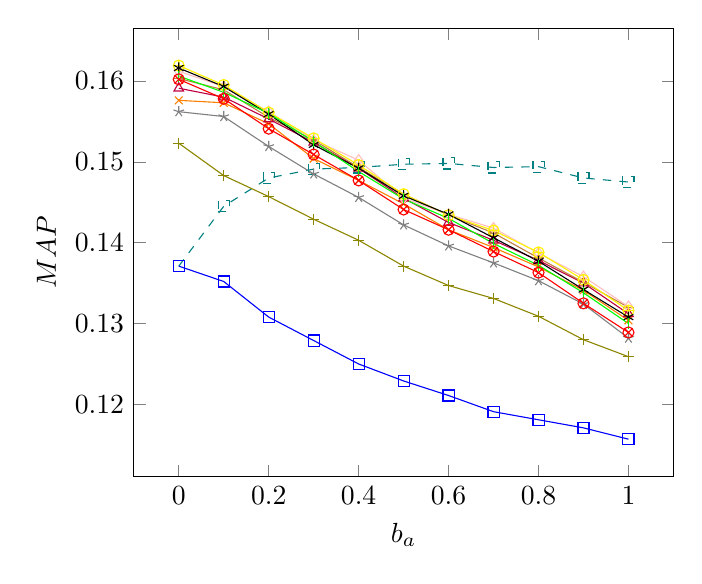
\begin{tikzpicture}
\begin{axis}[
xlabel=$b_a$,
ylabel=$MAP$,
% y label style={rotate=-90}
]

%%%%%%%%%%%
%% x = b_v, y = b_a
%%%%%%%%%%%
%\addplot[mark=square, style=solid, color=blue] coordinates
%{ (0.0,  0.1371 ) (0.1,  0.1523 ) (0.2,  0.1562 ) (0.3,  0.1576 ) (0.4,  0.1591 ) (0.5,  0.1603 ) (0.6,  0.1612 ) (0.7,  0.1619 ) (0.8,  0.1616 ) (0.9,  0.1606 ) (1.0,  0.1602 ) };

%\addplot[mark=+, style=solid, color=olive] coordinates
%{ (0.0,  0.1352 ) (0.1,  0.1483 ) (0.2,  0.1556 ) (0.3,  0.1573 ) (0.4,  0.158 ) (0.5,  0.1589 ) (0.6,  0.1593 ) (0.7,  0.1595 ) (0.8,  0.1593 ) (0.9,  0.1586 ) (1.0,  0.1578 ) };

%\addplot[mark=star, style=solid, color=gray] coordinates
%{ (0.0,  0.1308 ) (0.1,  0.1457 ) (0.2,  0.1519 ) (0.3,  0.1547 ) (0.4,  0.1553 ) (0.5,  0.1555 ) (0.6,  0.1562 ) (0.7,  0.1561 ) (0.8,  0.1559 ) (0.9,  0.156 ) (1.0,  0.1541 ) };

%\addplot[mark=x, style=solid, color=orange] coordinates
%{ (0.0,  0.1279 ) (0.1,  0.1429 ) (0.2,  0.1485 ) (0.3,  0.1504 ) (0.4,  0.1524 ) (0.5,  0.1527 ) (0.6,  0.1527 ) (0.7,  0.1529 ) (0.8,  0.1521 ) (0.9,  0.1525 ) (1.0,  0.1509 ) };

%\addplot[mark=triangle, style=solid, color=purple] coordinates
%{ (0.0,  0.125 ) (0.1,  0.1403 ) (0.2,  0.1456 ) (0.3,  0.1477 ) (0.4,  0.1492 ) (0.5,  0.1493 ) (0.6,  0.1502 ) (0.7,  0.1496 ) (0.8,  0.1492 ) (0.9,  0.1488 ) (1.0,  0.1477 ) };

%\addplot[mark=-, style=solid, color=brown] coordinates
%{ (0.0,  0.1229 ) (0.1,  0.1371 ) (0.2,  0.1422 ) (0.3,  0.1448 ) (0.4,  0.1455 ) (0.5,  0.146 ) (0.6,  0.1455 ) (0.7,  0.146 ) (0.8,  0.1458 ) (0.9,  0.1454 ) (1.0,  0.1441 ) };

%\addplot[mark=diamond, style=solid, color=pink] coordinates
%{ (0.0,  0.1211 ) (0.1,  0.1347 ) (0.2,  0.1396 ) (0.3,  0.1416 ) (0.4,  0.1425 ) (0.5,  0.1434 ) (0.6,  0.1435 ) (0.7,  0.1434 ) (0.8,  0.1435 ) (0.9,  0.143 ) (1.0,  0.1416 ) };

%\addplot[mark=oplus, style=solid, color=yellow] coordinates
%{ (0.0,  0.1191 ) (0.1,  0.1331 ) (0.2,  0.1375 ) (0.3,  0.1394 ) (0.4,  0.1403 ) (0.5,  0.1412 ) (0.6,  0.1418 ) (0.7,  0.1415 ) (0.8,  0.1406 ) (0.9,  0.1399 ) (1.0,  0.1389 ) };

%\addplot[mark=asterisk, style=solid, color=black] coordinates
%{ (0.0,  0.1181 ) (0.1,  0.1309 ) (0.2,  0.1353 ) (0.3,  0.137 ) (0.4,  0.1378 ) (0.5,  0.1381 ) (0.6,  0.1387 ) (0.7,  0.1388 ) (0.8,  0.1377 ) (0.9,  0.1372 ) (1.0,  0.1363 ) };

%\addplot[mark=|, style=solid, color=green] coordinates
%{ (0.0,  0.1171 ) (0.1,  0.128 ) (0.2,  0.1324 ) (0.3,  0.1341 ) (0.4,  0.135 ) (0.5,  0.1351 ) (0.6,  0.1358 ) (0.7,  0.1354 ) (0.8,  0.1342 ) (0.9,  0.1338 ) (1.0,  0.1325 ) };

%\addplot[mark=otimes, style=solid, color=red] coordinates
%{ (0.0,  0.1157 ) (0.1,  0.1259 ) (0.2,  0.1282 ) (0.3,  0.1304 ) (0.4,  0.1312 ) (0.5,  0.132 ) (0.6,  0.1321 ) (0.7,  0.1316 ) (0.8,  0.1308 ) (0.9,  0.13 ) (1.0,  0.1289 ) };

%%%%%%%%%%%
%% x = b_v, y = b_a
%%%%%%%%%%%
\addplot[mark=square, style=dashed, color=teal] coordinates
{ (0, 0.1371) (.1, 0.1445) (.2, 0.148) (.3, 0.1491) (.4, 0.1493) (.5, 0.1497) (.6, 0.1498) (.7, 0.1493) (.8, 0.1494) (.9, 0.148) (1.0, 0.1475) };

\addplot[mark=square, style=solid, color=blue] coordinates
{ (0.0, 0.1371) (0.1, 0.1352) (0.2, 0.1308) (0.3, 0.1279) (0.4, 0.125) (0.5, 0.1229) (0.6, 0.1211) (0.7, 0.1191) (0.8, 0.1181) (0.9, 0.1171) (1.0, 0.1157) };

\addplot[mark=+, style=solid, color=olive] coordinates
{ (0.0, 0.1523) (0.1, 0.1483) (0.2, 0.1457) (0.3, 0.1429) (0.4, 0.1403) (0.5, 0.1371) (0.6, 0.1347) (0.7, 0.1331) (0.8, 0.1309) (0.9, 0.128) (1.0, 0.1259) };

\addplot[mark=star, style=solid, color=gray] coordinates
{ (0.0, 0.1562) (0.1, 0.1556) (0.2, 0.1519) (0.3, 0.1485) (0.4, 0.1456) (0.5, 0.1422) (0.6, 0.1396) (0.7, 0.1375) (0.8, 0.1353) (0.9, 0.1324) (1.0, 0.1282) };

\addplot[mark=x, style=solid, color=orange] coordinates
{ (0.0, 0.1576) (0.1, 0.1573) (0.2, 0.1547) (0.3, 0.1504) (0.4, 0.1477) (0.5, 0.1448) (0.6, 0.1416) (0.7, 0.1394) (0.8, 0.137) (0.9, 0.1341) (1.0, 0.1304) };

\addplot[mark=triangle, style=solid, color=purple] coordinates
{ (0.0, 0.1591) (0.1, 0.158) (0.2, 0.1553) (0.3, 0.1524) (0.4, 0.1492) (0.5, 0.1455) (0.6, 0.1425) (0.7, 0.1403) (0.8, 0.1378) (0.9, 0.135) (1.0, 0.1312) };

\addplot[mark=-, style=solid, color=brown] coordinates
{ (0.0, 0.1603) (0.1, 0.1589) (0.2, 0.1555) (0.3, 0.1527) (0.4, 0.1493) (0.5, 0.146) (0.6, 0.1434) (0.7, 0.1412) (0.8, 0.1381) (0.9, 0.1351) (1.0, 0.132) };

\addplot[mark=diamond, style=solid, color=pink] coordinates
{ (0.0, 0.1612) (0.1, 0.1593) (0.2, 0.1562) (0.3, 0.1527) (0.4, 0.1502) (0.5, 0.1455) (0.6, 0.1435) (0.7, 0.1418) (0.8, 0.1387) (0.9, 0.1358) (1.0, 0.1321) };

\addplot[mark=oplus, style=solid, color=yellow] coordinates
{ (0.0, 0.1619) (0.1, 0.1595) (0.2, 0.1561) (0.3, 0.1529) (0.4, 0.1496) (0.5, 0.146) (0.6, 0.1434) (0.7, 0.1415) (0.8, 0.1388) (0.9, 0.1354) (1.0, 0.1316) };

\addplot[mark=asterisk, style=solid, color=black] coordinates
{ (0.0, 0.1616) (0.1, 0.1593) (0.2, 0.1559) (0.3, 0.1521) (0.4, 0.1492) (0.5, 0.1458) (0.6, 0.1435) (0.7, 0.1406) (0.8, 0.1377) (0.9, 0.1342) (1.0, 0.1308) };

\addplot[mark=|, style=solid, color=green] coordinates
{ (0.0, 0.1606) (0.1, 0.1586) (0.2, 0.156) (0.3, 0.1525) (0.4, 0.1488) (0.5, 0.1454) (0.6, 0.143) (0.7, 0.1399) (0.8, 0.1372) (0.9, 0.1338) (1.0, 0.13) };

\addplot[mark=otimes, style=solid, color=red] coordinates
{ (0.0, 0.1602) (0.1, 0.1578) (0.2, 0.1541) (0.3, 0.1509) (0.4, 0.1477) (0.5, 0.1441) (0.6, 0.1416) (0.7, 0.1389) (0.8, 0.1363) (0.9, 0.1325) (1.0, 0.1289) };

\end{axis}
\end{tikzpicture}}

	\caption{INEX09}
\end{subfigure}
\quad%
\begin{subfigure}[b]{.3\textwidth}
\centering
\resizebox{\textwidth}{!}{
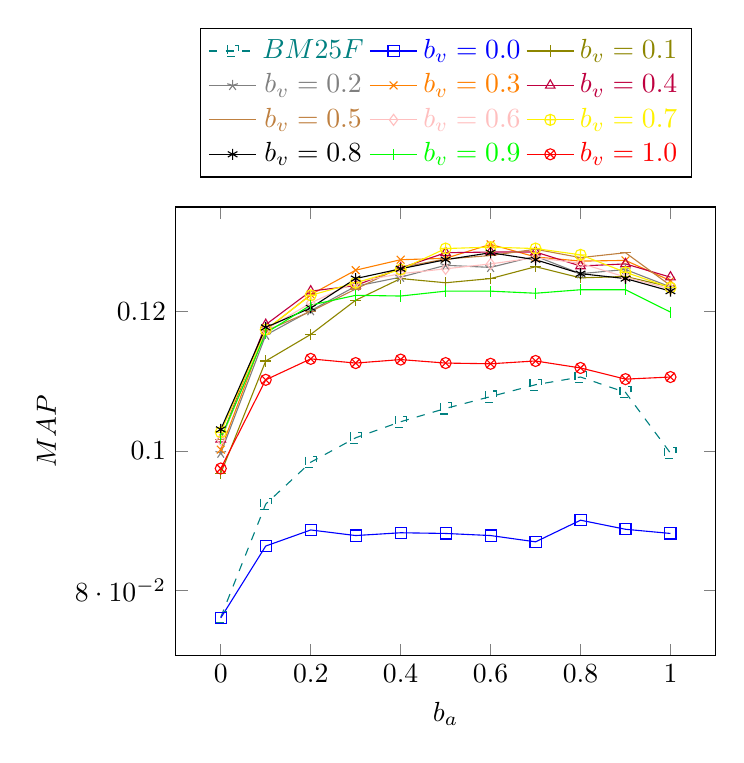
\begin{tikzpicture}
\begin{axis}[
  legend entries={
    [teal]$BM25F$,
	[blue]$b_v = 0.0$,
 	[olive]$b_v = 0.1$,
  	[gray]$b_v = 0.2$,
  	[orange]$b_v = 0.3$,
	[purple]$b_v = 0.4$,
 	[brown]$b_v = 0.5$,
  	[pink]$b_v = 0.6$,
  	[yellow]$b_v = 0.7$,
	[black]$b_v = 0.8$,
 	[green]$b_v = 0.9$,
 	[red]$b_v = 1.0$
  },
  legend columns=3,
legend style={at={(0.5,1.4)},anchor=north},
 xlabel=$b_a$,
ylabel=$MAP$,
% y label style={rotate=-90},
]

%%%%%%%%%%%
%% x = c_v, y = c_a
%%%%%%%%%%%
%\addplot[mark=square, style=solid, color=blue] coordinates
%{ (0.0, 0.0761) (0.1, 0.0968) (0.2, 0.0997) (0.3, 0.1002) (0.4, 0.1017) (0.5, 0.1016) (0.6, 0.1016) (0.7, 0.1027) (0.8, 0.1031) (0.9, 0.1018) (1.0, 0.0975) };

%\addplot[mark=+, style=solid, color=olive] coordinates
%{ (0.0, 0.0864) (0.1, 0.1129) (0.2, 0.1166) (0.3, 0.1173) (0.4, 0.1181) (0.5, 0.1172) (0.6, 0.1174) (0.7, 0.1174) (0.8, 0.1177) (0.9, 0.1169) (1.0, 0.1102) };

%\addplot[mark=star, style=solid, color=gray] coordinates
%{ (0.0, 0.0887) (0.1, 0.1167) (0.2, 0.1201) (0.3, 0.1224) (0.4, 0.1229) (0.5, 0.12) (0.6, 0.1212) (0.7, 0.1223) (0.8, 0.1205) (0.9, 0.1209) (1.0, 0.1132) };

%\addplot[mark=x, style=solid, color=orange] coordinates
%{ (0.0, 0.0879) (0.1, 0.1216) (0.2, 0.1236) (0.3, 0.1259) (0.4, 0.1237) (0.5, 0.1232) (0.6, 0.1242) (0.7, 0.1241) (0.8, 0.1247) (0.9, 0.1223) (1.0, 0.1126) };

%\addplot[mark=triangle, style=solid, color=purple] coordinates
%{ (0.0, 0.0883) (0.1, 0.1247) (0.2, 0.1249) (0.3, 0.1274) (0.4, 0.1262) (0.5, 0.1263) (0.6, 0.1254) (0.7, 0.126) (0.8, 0.1261) (0.9, 0.1222) (1.0, 0.1131) };

%\addplot[mark=-, style=solid, color=brown] coordinates
%{ (0.0, 0.0882) (0.1, 0.1241) (0.2, 0.1266) (0.3, 0.1276) (0.4, 0.1284) (0.5, 0.1275) (0.6, 0.1261) (0.7, 0.129) (0.8, 0.1274) (0.9, 0.1229) (1.0, 0.1126) };

%\addplot[mark=diamond, style=solid, color=pink] coordinates
%{ (0.0, 0.0879) (0.1, 0.1247) (0.2, 0.1263) (0.3, 0.1296) (0.4, 0.1285) (0.5, 0.128) (0.6, 0.1268) (0.7, 0.1292) (0.8, 0.1284) (0.9, 0.1229) (1.0, 0.1125) };

%\addplot[mark=oplus, style=solid, color=yellow] coordinates
%{ (0.0, 0.087) (0.1, 0.1264) (0.2, 0.1279) (0.3, 0.1278) (0.4, 0.1285) (0.5, 0.1289) (0.6, 0.1277) (0.7, 0.129) (0.8, 0.1274) (0.9, 0.1226) (1.0, 0.1129) };

%\addplot[mark=asterisk, style=solid, color=black] coordinates
%{ (0.0, 0.0901) (0.1, 0.1248) (0.2, 0.1254) (0.3, 0.1272) (0.4, 0.1265) (0.5, 0.1277) (0.6, 0.1269) (0.7, 0.1281) (0.8, 0.1254) (0.9, 0.1231) (1.0, 0.1119) };

%\addplot[mark=|, style=solid, color=green] coordinates
%{ (0.0, 0.0888) (0.1, 0.125) (0.2, 0.126) (0.3, 0.1273) (0.4, 0.1268) (0.5, 0.1284) (0.6, 0.1249) (0.7, 0.1256) (0.8, 0.1247) (0.9, 0.1231) (1.0, 0.1103) };

%\addplot[mark=otimes, style=solid, color=red] coordinates
%{ (0.0, 0.0882) (0.1, 0.1235) (0.2, 0.1235) (0.3, 0.1244) (0.4, 0.1249) (0.5, 0.1237) (0.6, 0.1232) (0.7, 0.1234) (0.8, 0.1229) (0.9, 0.1199) (1.0, 0.1106) };

%%%%%%%%%%%
%% x = b_a, y = b_v
%%%%%%%%%%%
\addplot[mark=square, style=dashed, color=teal] coordinates
{ (0, 0.0762) (.1, 0.0924) (.2, 0.0984) (.3, 0.1019) (.4, 0.1042) (.5, 0.1061) (.6, 0.1078) (.7, 0.1095) (.8, 0.1106) (.9, 0.1084) (1.0, 0.0997) };

\addplot[mark=square, style=solid, color=blue] coordinates
{ (0.0, 0.0761) (0.1, 0.0864) (0.2, 0.0887) (0.3, 0.0879) (0.4, 0.0883) (0.5, 0.0882) (0.6, 0.0879) (0.7, 0.087) (0.8, 0.0901) (0.9, 0.0888) (1.0, 0.0882) };

\addplot[mark=+, style=solid, color=olive] coordinates
{ (0.0, 0.0968) (0.1, 0.1129) (0.2, 0.1167) (0.3, 0.1216) (0.4, 0.1247) (0.5, 0.1241) (0.6, 0.1247) (0.7, 0.1264) (0.8, 0.1248) (0.9, 0.125) (1.0, 0.1235) };

\addplot[mark=star, style=solid, color=gray] coordinates
{ (0.0, 0.0997) (0.1, 0.1166) (0.2, 0.1201) (0.3, 0.1236) (0.4, 0.1249) (0.5, 0.1266) (0.6, 0.1263) (0.7, 0.1279) (0.8, 0.1254) (0.9, 0.126) (1.0, 0.1235) };

\addplot[mark=x, style=solid, color=orange] coordinates
{ (0.0, 0.1002) (0.1, 0.1173) (0.2, 0.1224) (0.3, 0.1259) (0.4, 0.1274) (0.5, 0.1276) (0.6, 0.1296) (0.7, 0.1278) (0.8, 0.1272) (0.9, 0.1273) (1.0, 0.1244) };

\addplot[mark=triangle, style=solid, color=purple] coordinates
{ (0.0, 0.1017) (0.1, 0.1181) (0.2, 0.1229) (0.3, 0.1237) (0.4, 0.1262) (0.5, 0.1284) (0.6, 0.1285) (0.7, 0.1285) (0.8, 0.1265) (0.9, 0.1268) (1.0, 0.1249) };

\addplot[mark=-, style=solid, color=brown] coordinates
{ (0.0, 0.1016) (0.1, 0.1172) (0.2, 0.12) (0.3, 0.1232) (0.4, 0.1263) (0.5, 0.1275) (0.6, 0.128) (0.7, 0.1289) (0.8, 0.1277) (0.9, 0.1284) (1.0, 0.1237) };

\addplot[mark=diamond, style=solid, color=pink] coordinates
{ (0.0, 0.1016) (0.1, 0.1174) (0.2, 0.1212) (0.3, 0.1242) (0.4, 0.1254) (0.5, 0.1261) (0.6, 0.1268) (0.7, 0.1277) (0.8, 0.1269) (0.9, 0.1249) (1.0, 0.1232) };

\addplot[mark=oplus, style=solid, color=yellow] coordinates
{ (0.0, 0.1027) (0.1, 0.1174) (0.2, 0.1223) (0.3, 0.1241) (0.4, 0.126) (0.5, 0.129) (0.6, 0.1292) (0.7, 0.129) (0.8, 0.1281) (0.9, 0.1256) (1.0, 0.1234) };

\addplot[mark=asterisk, style=solid, color=black] coordinates
{ (0.0, 0.1031) (0.1, 0.1177) (0.2, 0.1205) (0.3, 0.1247) (0.4, 0.1261) (0.5, 0.1274) (0.6, 0.1284) (0.7, 0.1274) (0.8, 0.1254) (0.9, 0.1247) (1.0, 0.1229) };

\addplot[mark=|, style=solid, color=green] coordinates
{ (0.0, 0.1018) (0.1, 0.1169) (0.2, 0.1209) (0.3, 0.1223) (0.4, 0.1222) (0.5, 0.1229) (0.6, 0.1229) (0.7, 0.1226) (0.8, 0.1231) (0.9, 0.1231) (1.0, 0.1199) };

\addplot[mark=otimes, style=solid, color=red] coordinates
{ (0.0, 0.0975) (0.1, 0.1102) (0.2, 0.1132) (0.3, 0.1126) (0.4, 0.1131) (0.5, 0.1126) (0.6, 0.1125) (0.7, 0.1129) (0.8, 0.1119) (0.9, 0.1103) (1.0, 0.1106) };

\end{axis}
\end{tikzpicture}}

	\caption{SS10}
\end{subfigure}
\quad%
\begin{subfigure}[b]{.3\textwidth}
\centering
\resizebox{\textwidth}{!}{
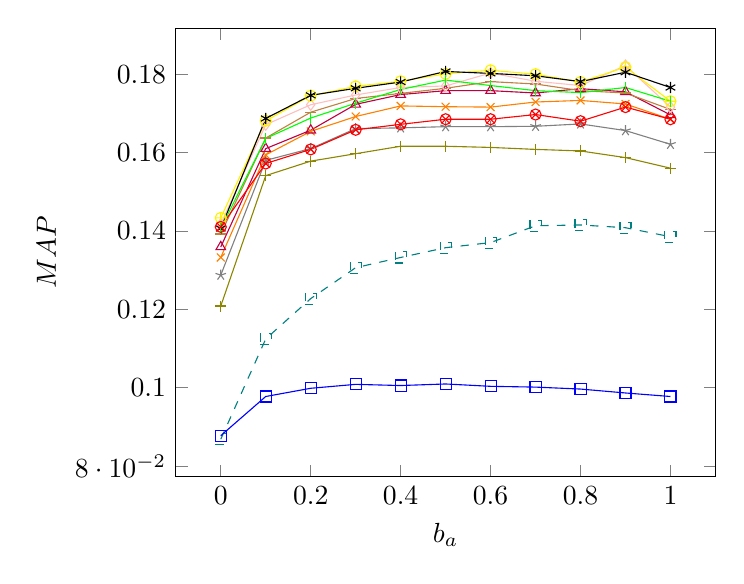
\begin{tikzpicture}
\begin{axis}[
 xlabel=$b_a$,
ylabel=$MAP$,
% y label style={rotate=-90},
]

%%%%%%%%%%%
%% x = b_v, y = b_a
%%%%%%%%%%%
%\addplot[mark=square, style=solid, color=blue] coordinates
%{ (0.0,  0.0877) (0.1,  0.1208) (0.2,  0.1287) (0.3,  0.1332) (0.4,  0.1359) (0.5,  0.1392) (0.6,  0.1417) (0.7,  0.1433) (0.8, 0.1406) (0.9, 0.1406) (1.0, 0.141) };

%\addplot[mark=+, style=solid, color=olive] coordinates
%{ (0.0,  0.0977) (0.1, 0.1541 ) (0.2,  0.158) (0.3, 0.1594) (0.4,  0.161) (0.5,  0.1637) (0.6, 0.1671) (0.7,  0.1681) (0.8, 0.1687) (0.9,  0.1636) (1.0,  0.1572) };

%\addplot[mark=star, style=solid, color=gray] coordinates
%{ (0.0, 0.0998 ) (0.1,  0.1578) (0.2,  0.161) (0.3,  0.1654) (0.4,  0.1657) (0.5, 0.1703) (0.6,  0.1722) (0.7, 0.1745) (0.8,  0.1746) (0.9,  0.1688) (1.0, 0.1608) };

%\addplot[mark=x, style=solid, color=orange] coordinates
%{ (0.0,  0.1008) (0.1,  0.1597) (0.2,  0.1661) (0.3,  0.1692) (0.4,  0.1723) (0.5, 0.1738) (0.6, 0.1747) (0.7, 0.1769) (0.8,  0.1764) (0.9,  0.1726) (1.0, 0.1658) };

%\addplot[mark=triangle, style=solid, color=purple] coordinates
%{ (0.0,  0.1005) (0.1,  0.1616) (0.2,  0.1663) (0.3,  0.1719) (0.4, 0.1748 ) (0.5, 0.1751) (0.6,0.1766 ) (0.7, 0.1782) (0.8,  0.178) (0.9,  0.1761) (1.0,  0.1672) };

%\addplot[mark=-, style=solid, color=brown] coordinates
%{ (0.0,  0.1009) (0.1,  0.1616) (0.2,  0.1666) (0.3,  0.1717) (0.4,  0.1758) (0.5, 0.1764 ) (0.6, 0.177) (0.7, 0.1801) (0.8,  0.1807) (0.9,  0.1785) (1.0, 0.1685) };

%\addplot[mark=diamond, style=solid, color=pink] coordinates
%{ (0.0,  0.1003) (0.1,  0.1613) (0.2,  0.1666) (0.3,  0.1716) (0.4,  0.1758) (0.5, 0.1781) (0.6, 0.1803) (0.7, 0.181) (0.8,  0.1802) (0.9,  0.1771) (1.0,  0.1685) };

%\addplot[mark=oplus, style=solid, color=yellow] coordinates
%{ (0.0,  0.1001) (0.1,  0.1608) (0.2,  0.1667) (0.3,  0.1729) (0.4,  0.1752) (0.5, 0.1775) (0.6, 0.1782) (0.7, 0.18) (0.8, 0.1796 ) (0.9,  0.1758) (1.0,  0.1697) };

%\addplot[mark=asterisk, style=solid, color=black] coordinates
%{ (0.0, 0.0996 ) (0.1,  0.1604) (0.2, 0.1673 ) (0.3, 0.1733 ) (0.4, 0.1763 ) (0.5, 0.1758 ) (0.6, 0.1771) (0.7, 0.178) (0.8,  0.1781) (0.9,  0.1753) (1.0,  0.168) };

%\addplot[mark=|, style=solid, color=green] coordinates
%{ (0.0,  0.0986) (0.1, 0.1587 ) (0.2, 0.1656 ) (0.3, 0.1724 ) (0.4, 0.1755 ) (0.5, 0.1752 ) (0.6, 0.1822) (0.7, 0.1818) (0.8, 0.1805 ) (0.9, 0.1766 ) (1.0, 0.1716 )
%};

%\addplot[mark=otimes, style=solid, color=red] coordinates
%{ (0.0, 0.0977 ) (0.1, 0.156 ) (0.2, 0.1621 ) (0.3, 0.1685 ) (0.4, 0.1696 ) (0.5, 0.171 ) (0.6, 0.1716 ) (0.7, 0.1731 ) (0.8, 0.1766) (0.9, 0.1731) (1.0, 0.1685 ) };

%%%%%%%%%%%
%% x = b_a, y = b_v
%%%%%%%%%%%

\addplot[mark=square, style=dashed, color=teal] coordinates
{ (0, 0.0868) (.1, 0.1124) (.2, 0.1227) (.3, 0.1306) (.4, 0.1332) (.5, 0.1357) (.6, 0.137) (.7, 0.1413) (.8, 0.1415) (.9, 0.1408) (1.0, 0.1385) };

\addplot[mark=square, style=solid, color=blue] coordinates
{ (0.0, 0.0877) (0.1, 0.0977) (0.2, 0.0998) (0.3, 0.1008) (0.4, 0.1005) (0.5, 0.1009) (0.6, 0.1003) (0.7, 0.1001) (0.8, 0.0996) (0.9, 0.0986) (1.0, 0.0977) };

\addplot[mark=+, style=solid, color=olive] coordinates
{ (0.0, 0.1208) (0.1, 0.1541) (0.2, 0.1578) (0.3, 0.1597) (0.4, 0.1616) (0.5, 0.1616) (0.6, 0.1613) (0.7, 0.1608) (0.8, 0.1604) (0.9, 0.1587) (1.0, 0.156) };

\addplot[mark=star, style=solid, color=gray] coordinates
{ (0.0, 0.1287) (0.1, 0.158) (0.2, 0.161) (0.3, 0.1661) (0.4, 0.1663) (0.5, 0.1666) (0.6, 0.1666) (0.7, 0.1667) (0.8, 0.1673) (0.9, 0.1656) (1.0, 0.1621) };

\addplot[mark=x, style=solid, color=orange] coordinates
{ (0.0, 0.1332) (0.1, 0.1594) (0.2, 0.1654) (0.3, 0.1692) (0.4, 0.1719) (0.5, 0.1717) (0.6, 0.1716) (0.7, 0.1729) (0.8, 0.1733) (0.9, 0.1724) (1.0, 0.1685) };

\addplot[mark=triangle, style=solid, color=purple] coordinates
{ (0.0, 0.1359) (0.1, 0.161) (0.2, 0.1657) (0.3, 0.1723) (0.4, 0.1748) (0.5, 0.1758) (0.6, 0.1758) (0.7, 0.1752) (0.8, 0.1763) (0.9, 0.1755) (1.0, 0.1696) };

\addplot[mark=-, style=solid, color=brown] coordinates
{ (0.0, 0.1392) (0.1, 0.1637) (0.2, 0.1703) (0.3, 0.1738) (0.4, 0.1751) (0.5, 0.1764) (0.6, 0.1781) (0.7, 0.1775) (0.8, 0.1758) (0.9, 0.1752) (1.0, 0.171) };

\addplot[mark=diamond, style=solid, color=pink] coordinates
{ (0.0, 0.1417) (0.1, 0.1671) (0.2, 0.1722) (0.3, 0.1747) (0.4, 0.1766) (0.5, 0.177) (0.6, 0.1803) (0.7, 0.1782) (0.8, 0.1771) (0.9, 0.1822) (1.0, 0.1716) };

\addplot[mark=oplus, style=solid, color=yellow] coordinates
{ (0.0, 0.1433) (0.1, 0.1681) (0.2, 0.1745) (0.3, 0.1769) (0.4, 0.1782) (0.5, 0.1801) (0.6, 0.181) (0.7, 0.18) (0.8, 0.178) (0.9, 0.1818) (1.0, 0.1731) };

\addplot[mark=asterisk, style=solid, color=black] coordinates
{ (0.0, 0.1406) (0.1, 0.1687) (0.2, 0.1746) (0.3, 0.1764) (0.4, 0.178) (0.5, 0.1807) (0.6, 0.1802) (0.7, 0.1796) (0.8, 0.1781) (0.9, 0.1805) (1.0, 0.1766) };

\addplot[mark=|, style=solid, color=green] coordinates
{ (0.0, 0.1406) (0.1, 0.1636) (0.2, 0.1688) (0.3, 0.1726) (0.4, 0.1761) (0.5, 0.1785) (0.6, 0.1771) (0.7, 0.1758) (0.8, 0.1753) (0.9, 0.1766) (1.0, 0.1731) };

\addplot[mark=otimes, style=solid, color=red] coordinates
{ (0.0, 0.141) (0.1, 0.1572) (0.2, 0.1608) (0.3, 0.1658) (0.4, 0.1672) (0.5, 0.1685) (0.6, 0.1685) (0.7, 0.1697) (0.8, 0.168) (0.9, 0.1716) (1.0, 0.1685) };

\end{axis}
\end{tikzpicture}}
\caption{SS11}
\end{subfigure}
\caption{Experiment with the BM25MF normalization parameters. The figures report the MAP values of the respective datasets, where a curve plots a fixed $b_v$ value with $b_a$ varying from $0$ to $1$ with a precision step of $0.1$.}
\label{fig:bm25mf-norm}
\end{figure}

		\addtocounter{subfigure}{-1}
		\caption{Evaluation of BM25MF normalization parameters. A curve plots a fixed $b_v$ value (Equation~(\ref{bm25mf_v})) with $b_a$ (Equation~(\ref{bm25mf_a})) varying from $0$ to $1$ with a precision step of $0.1$.}
		\label{fig:bm25mf-norm}
	\end{subfigure}
	\qquad
	\begin{subfigure}{\textwidth}
		\centering
		\begin{subfigure}[b]{.3\textwidth}
	\renewcommand\thesubfigure{\alph{subfigure}1}
	\centering
	\resizebox{\textwidth}{!}{
	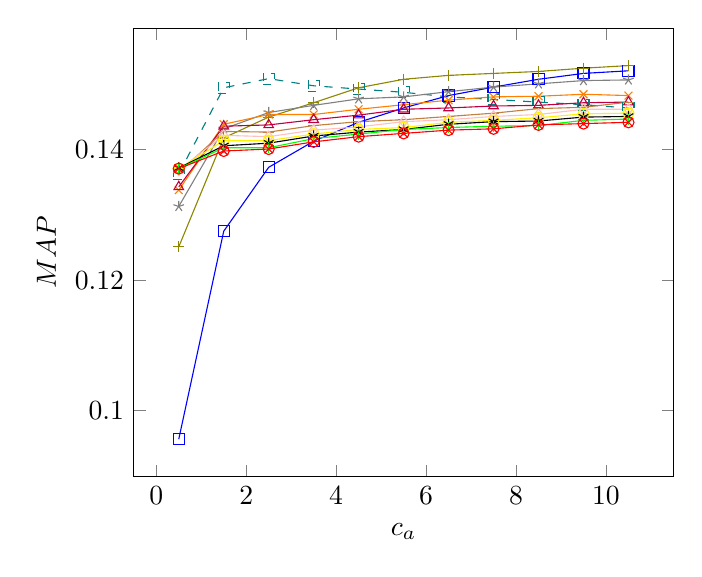
\begin{tikzpicture}
		\begin{axis}[
		xlabel=$c_a$,
		ylabel=$MAP$,
		% y label style={rotate=-90}
	]
%%%%%%%%%%%%%%%%%%%%
%%% x=cv y=ca, from 5 to 50, with step of 5
%%%%%%%%%%%%%%%%%%%%
%%\addplot[mark=square, style=solid, color=blue] coordinates

%\addplot[mark=+, style=solid, color=olive] coordinates
%{ (0, 0.1492) (5, 0.1451) (10, 0.1425) (15, 0.1411) (20, 0.1397) (25, 0.1381) (30, 0.1373) (35, 0.137) (40, 0.1365) (45, 0.136) (50, 0.1356) };

%\addplot[mark=star, style=solid, color=gray] coordinates
%{ (0, 0.1468) (5, 0.1469) (10, 0.1444) (15, 0.1421) (20, 0.1408) (25, 0.1397) (30, 0.1387) (35, 0.1381) (40, 0.1377) (45, 0.1372) (50, 0.1369) };

%\addplot[mark=x, style=solid, color=orange] coordinates
%{ (0, 0.1452) (5, 0.1476) (10, 0.1442) (15, 0.1419) (20, 0.1407) (25, 0.1397) (30, 0.1388) (35, 0.1382) (40, 0.1377) (45, 0.1373) (50, 0.1369) };

%\addplot[mark=triangle, style=solid, color=purple] coordinates
%{ (0, 0.1443) (5, 0.1475) (10, 0.1435) (15, 0.1415) (20, 0.1403) (25, 0.1393) (30, 0.1384) (35, 0.1379) (40, 0.1375) (45, 0.1371) (50, 0.1369) };

%\addplot[mark=-, style=solid, color=brown] coordinates
%{ (0, 0.1431) (5, 0.1472) (10, 0.1435) (15, 0.1413) (20, 0.1399) (25, 0.139) (30, 0.1384) (35, 0.1378) (40, 0.1374) (45, 0.1371) (50, 0.1367) };

%\addplot[mark=diamond, style=solid, color=pink] coordinates
%{ (0, 0.1422) (5, 0.1472) (10, 0.1432) (15, 0.1412) (20, 0.1401) (25, 0.1393) (30, 0.1385) (35, 0.1379) (40, 0.1376) (45, 0.1372) (50, 0.137) };

%\addplot[mark=oplus, style=solid, color=yellow] coordinates
%{ (0, 0.1418) (5, 0.1473) (10, 0.1431) (15, 0.1411) (20, 0.1401) (25, 0.1392) (30, 0.1387) (35, 0.1383) (40, 0.1378) (45, 0.1374) (50, 0.137) };

%\addplot[mark=asterisk, style=solid, color=black] coordinates
%{ (0, 0.141) (5, 0.147) (10, 0.1431) (15, 0.1411) (20, 0.1402) (25, 0.1392) (30, 0.1389) (35, 0.1383) (40, 0.1378) (45, 0.1373) (50, 0.137) };

%\addplot[mark=|, style=solid, color=green] coordinates
%{ (0, 0.1406) (5, 0.1468) (10, 0.143) (15, 0.1413) (20, 0.1403) (25, 0.1394) (30, 0.1387) (35, 0.1382) (40, 0.1377) (45, 0.1372) (50, 0.1369) };

%\addplot[mark=otimes, style=solid, color=red] coordinates
%{ (0, 0.1403) (5, 0.1466) (10, 0.1431) (15, 0.1412) (20, 0.1402) (25, 0.1394) (30, 0.1386) (35, 0.1383) (40, 0.1379) (45, 0.1373) (50, 0.1368) };

%%%%%%%%%%%%%%%%%%%%
%%% x=ca y=cv, from 0.5 to 10.5, with step of 1
%%%%%%%%%%%%%%%%%%%%
\addplot[mark=square, style=dashed, color=teal] coordinates
{ (0.5, 0.1363) (1.5, 0.1495) (2.5, 0.1509) (3.5, 0.1498) (4.5, 0.1493) (5.5, 0.1488) (6.5, 0.1481) (7.5, 0.1477) (8.5, 0.1473) (9.5, 0.1469) (10.5, 0.1464) };

\addplot[mark=square, style=solid, color=blue] coordinates
{ (0.5, 0.0956) (1.5, 0.1275) (2.5, 0.1373) (3.5, 0.1413) (4.5, 0.1442) (5.5, 0.1464) (6.5, 0.1483) (7.5, 0.1496) (8.5, 0.1508) (9.5, 0.1517) (10.5, 0.1521) };

\addplot[mark=+, style=solid, color=olive] coordinates
{ (0.5, 0.1251) (1.5, 0.1418) (2.5, 0.145) (3.5, 0.1472) (4.5, 0.1495) (5.5, 0.1508) (6.5, 0.1514) (7.5, 0.1517) (8.5, 0.152) (9.5, 0.1525) (10.5, 0.1529) };

\addplot[mark=star, style=solid, color=gray] coordinates
{ (0.5, 0.1313) (1.5, 0.1432) (2.5, 0.1457) (3.5, 0.1468) (4.5, 0.1478) (5.5, 0.1481) (6.5, 0.1489) (7.5, 0.1496) (8.5, 0.1501) (9.5, 0.1506) (10.5, 0.1507) };

\addplot[mark=x, style=solid, color=orange] coordinates
{ (0.5, 0.1338) (1.5, 0.1439) (2.5, 0.1454) (3.5, 0.1454) (4.5, 0.1462) (5.5, 0.1469) (6.5, 0.1476) (7.5, 0.1481) (8.5, 0.1482) (9.5, 0.1485) (10.5, 0.1483) };

\addplot[mark=triangle, style=solid, color=purple] coordinates
{ (0.5, 0.1343) (1.5, 0.1436) (2.5, 0.1438) (3.5, 0.1446) (4.5, 0.1453) (5.5, 0.1462) (6.5, 0.1464) (7.5, 0.1467) (8.5, 0.1468) (9.5, 0.1472) (10.5, 0.1473) };

\addplot[mark=-, style=solid, color=brown] coordinates
{ (0.5, 0.1365) (1.5, 0.1428) (2.5, 0.1427) (3.5, 0.1437) (4.5, 0.1443) (5.5, 0.1446) (6.5, 0.1451) (7.5, 0.1456) (8.5, 0.1463) (9.5, 0.1465) (10.5, 0.1473) };

\addplot[mark=diamond, style=solid, color=pink] coordinates
{ (0.5, 0.1369) (1.5, 0.1422) (2.5, 0.142) (3.5, 0.143) (4.5, 0.1435) (5.5, 0.1443) (6.5, 0.1446) (7.5, 0.1451) (8.5, 0.1454) (9.5, 0.1462) (10.5, 0.1462) };

\addplot[mark=oplus, style=solid, color=yellow] coordinates
{ (0.5, 0.1371) (1.5, 0.1414) (2.5, 0.1414) (3.5, 0.1424) (4.5, 0.1431) (5.5, 0.1434) (6.5, 0.1442) (7.5, 0.1445) (8.5, 0.1449) (9.5, 0.1455) (10.5, 0.1456) };

\addplot[mark=asterisk, style=solid, color=black] coordinates
{ (0.5, 0.1372) (1.5, 0.1406) (2.5, 0.141) (3.5, 0.1421) (4.5, 0.1427) (5.5, 0.1431) (6.5, 0.1439) (7.5, 0.1443) (8.5, 0.1444) (9.5, 0.145) (10.5, 0.1451) };

\addplot[mark=|, style=solid, color=green] coordinates
{ (0.5, 0.1371) (1.5, 0.1403) (2.5, 0.1403) (3.5, 0.1417) (4.5, 0.1424) (5.5, 0.1431) (6.5, 0.1434) (7.5, 0.1436) (8.5, 0.1437) (9.5, 0.1445) (10.5, 0.1447) };

\addplot[mark=otimes, style=solid, color=red] coordinates
{ (0.5, 0.1371) (1.5, 0.1398) (2.5, 0.1401) (3.5, 0.1412) (4.5, 0.142) (5.5, 0.1425) (6.5, 0.143) (7.5, 0.1432) (8.5, 0.1438) (9.5, 0.144) (10.5, 0.1442) };

\end{axis}
\end{tikzpicture}}

	\caption{INEX09}
\end{subfigure}
\quad%
\begin{subfigure}[b]{.3\textwidth}
	\addtocounter{subfigure}{-1}
	\renewcommand\thesubfigure{\alph{subfigure}2}
	\centering
	\resizebox{\textwidth}{!}{
	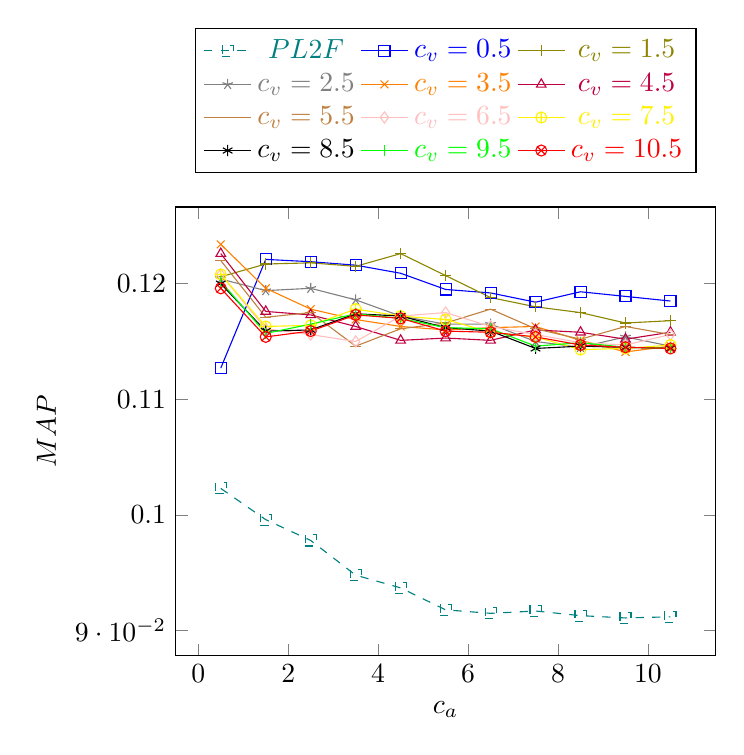
\begin{tikzpicture}
	\begin{axis}[
	  legend entries={
	    [teal]$PL2F$,
		[blue]$c_v = 0.5$,
	 	[olive]$c_v = 1.5$,
	  	[gray]$c_v = 2.5$,
	  	[orange]$c_v = 3.5$,
		[purple]$c_v = 4.5$,
	 	[brown]$c_v = 5.5$,
	  	[pink]$c_v = 6.5$,
	  	[yellow]$c_v = 7.5$,
		[black]$c_v = 8.5$,
	 	[green]$c_v = 9.5$,
	 	[red]$c_v = 10.5$
	  },
	  legend columns=3,
	legend style={at={(0.5,1.4)},anchor=north},
	 xlabel=$c_a$,
	ylabel=$MAP$,
	% y label style={rotate=-90},
	]

%%%%%%%%%%%%%%%%%%%%
%%% x=cv y=ca, from 5 to 50, with step of 5
%%%%%%%%%%%%%%%%%%%%
%\addplot[mark=square, style=solid, color=blue] coordinates
%{ (5, ) (10, ) (15, ) (20, ) (25, ) (30, ) (35, ) (40, ) (45, ) (50, )  };

%\addplot[mark=+, style=solid, color=olive] coordinates
%{ (0, 0.0928) (5, 0.1153) (10, 0.1174) (15, 0.116) (20, 0.1167) (25, 0.115) (30, 0.1136) (35, 0.1137) (40, 0.1139) (45, 0.1132) (50, 0.1136)  };

%\addplot[mark=star, style=solid, color=gray] coordinates
%{ (0, 0.0913) (5, 0.1158) (10, 0.1144) (15, 0.113) (20, 0.1136) (25, 0.114) (30, 0.1126) (35, 0.1127) (40, 0.112) (45, 0.1114) (50, 0.1106)  };

%\addplot[mark=x, style=solid, color=orange] coordinates
%{ (0, 0.0886) (5, 0.115) (10, 0.114) (15, 0.1127) (20, 0.1123) (25, 0.1123) (30, 0.1122) (35, 0.1121) (40, 0.1113) (45, 0.1105) (50, 0.1104)  };

%\addplot[mark=triangle, style=solid, color=purple] coordinates
%{ (0, 0.0879) (5, 0.114) (10, 0.1132) (15, 0.112) (20, 0.1124) (25, 0.1119) (30, 0.111) (35, 0.1111) (40, 0.1097) (45, 0.1097) (50, 0.1098)  };

%\addplot[mark=-, style=solid, color=brown] coordinates
%{ (0, 0.0868) (5, 0.1137) (10, 0.1137) (15, 0.1125) (20, 0.1111) (25, 0.1105) (30, 0.1101) (35, 0.11) (40, 0.1099) (45, 0.109) (50, 0.1091)  };

%\addplot[mark=diamond, style=solid, color=pink] coordinates
%{ (0, 0.0864) (5, 0.1131) (10, 0.1126) (15, 0.111) (20, 0.1104) (25, 0.1092) (30, 0.1092) (35, 0.1093) (40, 0.109) (45, 0.1081) (50, 0.1082)  };

%\addplot[mark=oplus, style=solid, color=yellow] coordinates
%{ (0, 0.0856) (5, 0.1129) (10, 0.1109) (15, 0.1105) (20, 0.1097) (25, 0.1084) (30, 0.1082) (35, 0.1076) (40, 0.1081) (45, 0.1079) (50, 0.107)  };

%\addplot[mark=asterisk, style=solid, color=black] coordinates
%{ (0, 0.0845) (5, 0.1124) (10, 0.1115) (15, 0.1102) (20, 0.1095) (25, 0.1083) (30, 0.1079) (35, 0.1078) (40, 0.1075) (45, 0.1073) (50, 0.1066)  };

%\addplot[mark=|, style=solid, color=green] coordinates
%{ (0, 0.0833) (5, 0.1121) (10, 0.1113) (15, 0.1099) (20, 0.1095) (25, 0.1087) (30, 0.1081) (35, 0.1081) (40, 0.1077) (45, 0.1068) (50, 0.1059)  };

%\addplot[mark=otimes, style=solid, color=red] coordinates
%{ (0, 0.0824) (5, 0.1116) (10, 0.1109) (15, 0.1099) (20, 0.1095) (25, 0.1086) (30, 0.1077) (35, 0.1077) (40, 0.1076) (45, 0.107) (50, 0.1068)  };

%%%%%%%%%%%%%%%%%%%%
%%% x=ca y=cv, from 0.5 to 10.5, with step of 1
%%%%%%%%%%%%%%%%%%%%
\addplot[mark=square, style=dashed, color=teal] coordinates
{ (0.5, 0.1023) (1.5, 0.0996) (2.5, 0.0978) (3.5, 0.0948) (4.5, 0.0937) (5.5, 0.0918) (6.5, 0.0915) (7.5, 0.0917) (8.5, 0.0913) (9.5, 0.0911) (10.5, 0.0912) };

\addplot[mark=square, style=solid, color=blue] coordinates
{ (0.5, 0.1127) (1.5, 0.1221) (2.5, 0.1219) (3.5, 0.1216) (4.5, 0.1209) (5.5, 0.1195) (6.5, 0.1192) (7.5, 0.1184) (8.5, 0.1193) (9.5, 0.1189) (10.5, 0.1185) };

\addplot[mark=+, style=solid, color=olive] coordinates
{ (0.5, 0.1206) (1.5, 0.1217) (2.5, 0.1218) (3.5, 0.1215) (4.5, 0.1226) (5.5, 0.1207) (6.5, 0.1188) (7.5, 0.118) (8.5, 0.1175) (9.5, 0.1166) (10.5, 0.1168) };

\addplot[mark=star, style=solid, color=gray] coordinates
{ (0.5, 0.1204) (1.5, 0.1194) (2.5, 0.1196) (3.5, 0.1186) (4.5, 0.1172) (5.5, 0.1165) (6.5, 0.1165) (7.5, 0.115) (8.5, 0.1145) (9.5, 0.1154) (10.5, 0.1146) };

\addplot[mark=x, style=solid, color=orange] coordinates
{ (0.5, 0.1234) (1.5, 0.1196) (2.5, 0.1178) (3.5, 0.1169) (4.5, 0.1163) (5.5, 0.116) (6.5, 0.1162) (7.5, 0.1163) (8.5, 0.1151) (9.5, 0.1141) (10.5, 0.1146) };

\addplot[mark=triangle, style=solid, color=purple] coordinates
{ (0.5, 0.1226) (1.5, 0.1176) (2.5, 0.1173) (3.5, 0.1163) (4.5, 0.1151) (5.5, 0.1153) (6.5, 0.1151) (7.5, 0.116) (8.5, 0.1158) (9.5, 0.1152) (10.5, 0.1158) };

\addplot[mark=-, style=solid, color=brown] coordinates
{ (0.5, 0.122) (1.5, 0.1171) (2.5, 0.1175) (3.5, 0.1146) (4.5, 0.1161) (5.5, 0.1166) (6.5, 0.1178) (7.5, 0.1161) (8.5, 0.1152) (9.5, 0.1163) (10.5, 0.1156) };

\addplot[mark=diamond, style=solid, color=pink] coordinates
{ (0.5, 0.1208) (1.5, 0.1161) (2.5, 0.1156) (3.5, 0.115) (4.5, 0.1172) (5.5, 0.1175) (6.5, 0.1163) (7.5, 0.1156) (8.5, 0.1149) (9.5, 0.1147) (10.5, 0.1156) };

\addplot[mark=oplus, style=solid, color=yellow] coordinates
{ (0.5, 0.1208) (1.5, 0.1163) (2.5, 0.1164) (3.5, 0.1178) (4.5, 0.1172) (5.5, 0.1169) (6.5, 0.1158) (7.5, 0.1154) (8.5, 0.1143) (9.5, 0.1144) (10.5, 0.1147) };

\addplot[mark=asterisk, style=solid, color=black] coordinates
{ (0.5, 0.12) (1.5, 0.1159) (2.5, 0.116) (3.5, 0.1174) (4.5, 0.1172) (5.5, 0.1162) (6.5, 0.1159) (7.5, 0.1144) (8.5, 0.1146) (9.5, 0.1145) (10.5, 0.1144) };

\addplot[mark=|, style=solid, color=green] coordinates
{ (0.5, 0.1202) (1.5, 0.1157) (2.5, 0.1165) (3.5, 0.1174) (4.5, 0.117) (5.5, 0.1162) (6.5, 0.1161) (7.5, 0.1146) (8.5, 0.1149) (9.5, 0.1145) (10.5, 0.1144) };

\addplot[mark=otimes, style=solid, color=red] coordinates
{ (0.5, 0.1196) (1.5, 0.1154) (2.5, 0.1159) (3.5, 0.1173) (4.5, 0.117) (5.5, 0.1159) (6.5, 0.1158) (7.5, 0.1154) (8.5, 0.1147) (9.5, 0.1145) (10.5, 0.1144) };

\end{axis}
\end{tikzpicture}}

	\caption{SS10}
\end{subfigure}
\quad%
\begin{subfigure}[b]{.3\textwidth}
	\addtocounter{subfigure}{-1}
	\renewcommand\thesubfigure{\alph{subfigure}3}
	\centering
	\resizebox{\textwidth}{!}{
	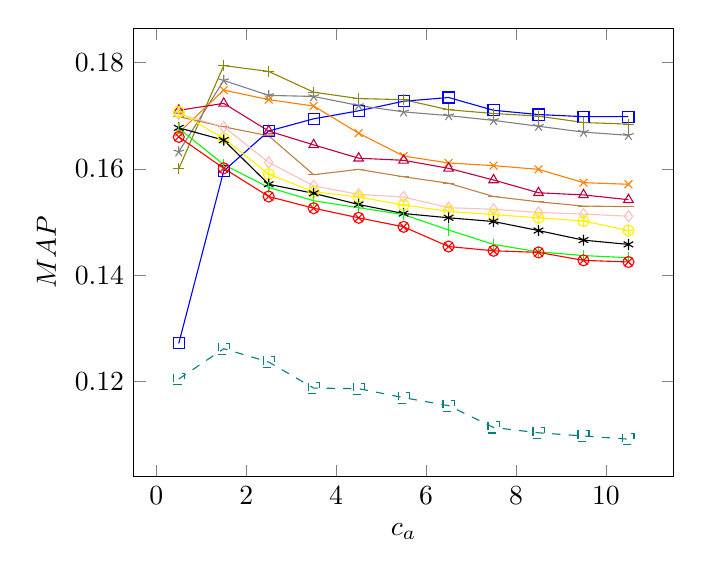
\begin{tikzpicture}
	\begin{axis}[
	 xlabel=$c_a$,
	ylabel=$MAP$,
	% y label style={rotate=-90},
	]

%%%%%%%%%%%%%%%%%%%%
%%% x=cv y=ca, from 5 to 50, with step of 5
%%%%%%%%%%%%%%%%%%%%
%%\addplot[mark=square, style=solid, color=blue] coordinates
%%{ ( , ) ( , ) ( , ) ( , ) ( , ) ( , ) ( , ) ( , ) ( , ) ( , ) ( , ) };

%\addplot[mark=+, style=solid, color=olive] coordinates
%{ (0, 0.1171) (5, 0.1608) (10 , 0.1506) (15 , 0.1448) (20 , 0.14) (25 , 0.1398) (30 , 0.139) (35 , 0.1381) (40 , 0.1371) (45 , 0.1368) (50 , 0.1361) };

%\addplot[mark=star, style=solid, color=gray] coordinates
%{ (0, 0.1098) (5 , 0.1539) (10 , 0.1436) (15 , 0.1378) (20 , 0.137) (25 , 0.1364) (30 , 0.136) (35 , 0.1351) (40 , 0.1347) (45 , 0.1342) (50 , 0.1338) };

%\addplot[mark=x, style=solid, color=orange] coordinates
%{ (0, 0.1073) (5, 0.1511) (10 , 0.1385) (15 , 0.1357) (20 , 0.1342) (25 , 0.1334) (30 , 0.1326) (35 , 0.132) (40 , 0.1312) (45 , 0.1308) (50 , 0.1282) };

%\addplot[mark=triangle, style=solid, color=purple] coordinates
%{ (0, 0.104) (5, 0.1483) (10 , 0.1365) (15 , 0.1337) (20 , 0.1327) (25 , 0.1322) (30 , 0.1312) (35 , 0.1311) (40 , 0.13) (45 , 0.1278) (50 , 0.1279) };

%\addplot[mark=-, style=solid, color=brown] coordinates
%{ (0, 0.1031) (5, 0.1464) (10 , 0.1347) (15 , 0.1327) (20 , 0.1317) (25 , 0.1314) (30 , 0.1306) (35 , 0.1302) (40 , 0.1295) (45 , 0.1274) (50 , 0.1269) };

%\addplot[mark=diamond, style=solid, color=pink] coordinates
%{ (0, 0.1024) (5, 0.1442) (10, 0.134) (15, 0.1321) (20, 0.1311) (25, 0.1309) (30, 0.1304) (35, 0.1293) (40, 0.1271) (45, 0.1268) (50, 0.1256) };

%\addplot[mark=oplus, style=solid, color=yellow] coordinates
%{ (0, 0.1019) (5, 0.1431) (10, 0.1331) (15, 0.1316) (20, 0.131) (25, 0.1304) (30, 0.1296) (35, 0.129) (40, 0.1265) (45, 0.126) (50, 0.1256) };

%\addplot[mark=asterisk, style=solid, color=black] coordinates
%{ (0, 0.1002) (5, 0.1428) (10, 0.1326) (15, 0.1311) (20, 0.1301) (25, 0.1298) (30, 0.1288) (35, 0.1285) (40, 0.1261) (45, 0.1258) (50, 0.1252) };

%\addplot[mark=|, style=solid, color=green] coordinates
%{ (0, 0.0988) (5, 0.1418) (10, 0.1322) (15, 0.1303) (20, 0.1293) (25, 0.1293) (30, 0.1284) (35, 0.1262) (40, 0.1253) (45, 0.1251) (50, 0.1247) };

%\addplot[mark=otimes, style=solid, color=red] coordinates
%{ (0, 0.0956) (5, 0.1415) (10, 0.1319) (15, 0.1301) (20, 0.129) (25, 0.1287) (30, 0.1279) (35, 0.1254) (40, 0.1251) (45, 0.1249) (50, 0.1242) };

%%%%%%%%%%%%%%%%%%%%
%%% x=ca y=cv, from 0.5 to 10.5, with step of 1
%%%%%%%%%%%%%%%%%%%%
\addplot[mark=square, style=dashed, color=teal] coordinates
{ (0.5, 0.1205) (1.5, 0.1262) (2.5, 0.1237) (3.5, 0.1188) (4.5, 0.1187) (5.5, 0.117) (6.5, 0.1155) (7.5, 0.1114) (8.5, 0.1104) (9.5, 0.1098) (10.5, 0.1092) };

\addplot[mark=square, style=solid, color=blue] coordinates
{ (0.5, 0.1272) (1.5, 0.1596) (2.5, 0.1671) (3.5, 0.1694) (4.5, 0.1709) (5.5, 0.1727) (6.5, 0.1734) (7.5, 0.171) (8.5, 0.1702) (9.5, 0.1698) (10.5, 0.1698) };

\addplot[mark=+, style=solid, color=olive] coordinates
{ (0.5, 0.16) (1.5, 0.1794) (2.5, 0.1783) (3.5, 0.1744) (4.5, 0.1732) (5.5, 0.173) (6.5, 0.1711) (7.5, 0.1704) (8.5, 0.1699) (9.5, 0.1687) (10.5, 0.1684) };

\addplot[mark=star, style=solid, color=gray] coordinates
{ (0.5, 0.1632) (1.5, 0.1766) (2.5, 0.1738) (3.5, 0.1736) (4.5, 0.1719) (5.5, 0.1707) (6.5, 0.17) (7.5, 0.1691) (8.5, 0.168) (9.5, 0.1669) (10.5, 0.1663) };

\addplot[mark=x, style=solid, color=orange] coordinates
{ (0.5, 0.1668) (1.5, 0.1748) (2.5, 0.173) (3.5, 0.1718) (4.5, 0.1667) (5.5, 0.1624) (6.5, 0.1611) (7.5, 0.1606) (8.5, 0.1599) (9.5, 0.1574) (10.5, 0.1571) };

\addplot[mark=triangle, style=solid, color=purple] coordinates
{ (0.5, 0.171) (1.5, 0.1723) (2.5, 0.1671) (3.5, 0.1645) (4.5, 0.162) (5.5, 0.1616) (6.5, 0.1601) (7.5, 0.1579) (8.5, 0.1555) (9.5, 0.1551) (10.5, 0.1542) };

\addplot[mark=-, style=solid, color=brown] coordinates
{ (0.5, 0.1698) (1.5, 0.1679) (2.5, 0.1662) (3.5, 0.1589) (4.5, 0.1599) (5.5, 0.1585) (6.5, 0.1573) (7.5, 0.1548) (8.5, 0.1538) (9.5, 0.153) (10.5, 0.1529) };

\addplot[mark=diamond, style=solid, color=pink] coordinates
{ (0.5, 0.1703) (1.5, 0.1679) (2.5, 0.1612) (3.5, 0.1568) (4.5, 0.1552) (5.5, 0.1547) (6.5, 0.1527) (7.5, 0.1524) (8.5, 0.1518) (9.5, 0.1515) (10.5, 0.1511) };

\addplot[mark=oplus, style=solid, color=yellow] coordinates
{ (0.5, 0.1707) (1.5, 0.1657) (2.5, 0.159) (3.5, 0.1557) (4.5, 0.1547) (5.5, 0.1532) (6.5, 0.152) (7.5, 0.1514) (8.5, 0.1508) (9.5, 0.1502) (10.5, 0.1484) };

\addplot[mark=asterisk, style=solid, color=black] coordinates
{ (0.5, 0.1677) (1.5, 0.1654) (2.5, 0.1571) (3.5, 0.1554) (4.5, 0.1533) (5.5, 0.1516) (6.5, 0.1508) (7.5, 0.1501) (8.5, 0.1484) (9.5, 0.1466) (10.5, 0.1458) };

\addplot[mark=|, style=solid, color=green] coordinates
{ (0.5, 0.1676) (1.5, 0.1608) (2.5, 0.1565) (3.5, 0.154) (4.5, 0.1527) (5.5, 0.1514) (6.5, 0.1485) (7.5, 0.1458) (8.5, 0.1444) (9.5, 0.1437) (10.5, 0.1433) };

\addplot[mark=otimes, style=solid, color=red] coordinates
{ (0.5, 0.166) (1.5, 0.1601) (2.5, 0.1548) (3.5, 0.1526) (4.5, 0.1508) (5.5, 0.1491) (6.5, 0.1454) (7.5, 0.1446) (8.5, 0.1443) (9.5, 0.1428) (10.5, 0.1425) };

\end{axis}
\end{tikzpicture}}

	\centering
	\caption{SS11}
\end{subfigure}

		\addtocounter{subfigure}{-1}
		\caption{Evaluation of PL2MF normalization parameters. A curve plots a fixed $c_v$ value (Equation~(\ref{eq:pl2mf_v})) with $c_a$ (Equation~(\ref{eq:pl2mf_a})) varying from $0.5$ to $10.5$ with a precision step of $1$.}
		\label{fig:pl2mf-norm}
	\end{subfigure}
	\caption{Impact of the normalisation parameters on the MF ranking functions. The figures report the MAP values of the respective datasets on the Y axis. On the X axis and with each curve, we vary the values of normalisation parameters.}
\end{figure}

\subsection{Comparison between MF and Field-Based Models}
\label{sec:mf-field-cmp}

In this section, we evaluate and compare the performance of BM25 and PL2 ranking model against their MF extensions, BM25MF and PL2F respectively, and show the superiority of the MF model. The TF-IDF function is used as a baseline.

\begin{labeling}{\emph{BM25~\cite{robertson:1994:sigir}}}
  \item[\emph{TF-IDF}] is a logarithmic function of the term frequency and defines the Equation (\ref{eq:tfidf-score}) as
  $
  tfn=log(F_t)+1
  $,
  where $F_t$ is the number of occurrences of the term $t$ in the entity.
  \item[\emph{BM25~\cite{robertson:1994:sigir}}] considers the document as a simple bag of words. It is a function of the term frequency derived from a two-Poisson model and it uses an entity-length normalization. The entity length is computed as the sum of the \emph{field length} defined in the Section~\ref{sec:ranking-wod}.

  It defines the Equation (\ref{eq:tfidf-score}) as
  $
  tfn=\frac{F_t\times(k_1+1)}{F_t+k_1\times \left(1+b\times\left(\frac{l_e}{l_{avg}}-1\right)\right)}
  $,
where $l_e$ is the \emph{entity length} of the entity $e$, $l_{avg}$ is the average of the \emph{entity length} in the collection and $b$ is a normalization parameter.
  \item[\emph{BM25F}] is defined in Equation (\ref{eq:tfidf-score}). It considers documents as composed of fields, each field being a bag of words.
  \item[\emph{PL2~\cite{amati:2002:acm}}] considers the document as a simple bag of words. It is a model derived from the DFR framework, with the Equation (\ref{eq:pl2f}) formulated as
  $
  tfn=F_t\times log_2\left(1+c\times\frac{l_{avg}}{l_e}\right)
  $,
  where $c$ is a normalization parameter.
  \item[\emph{PL2F}] is defined in Equation (\ref{eq:dfr-score}). It considers a document as a set of fields, each field being a bag of words.
\end{labeling}

The Table~\ref{tab:norm-param} reports the values of normalization parameters for each ranking function. For a given function and dataset, the parameter value that maximises the Mean Average Precision (MAP) is found through a constrained particle swarm optimisation~\cite{xiaohui:2002:sci}. The optimisation is run on ranking functions that have all their weights equal to one, i.e., $\alpha_e = \alpha_a = \alpha_v = 1$.\\

\begin{table}
	\centering
	\ra{0.5}
	\resizebox{\textwidth}{!}{
		\begin{tabular}{lc@{\hs}llrcllrc@{\hs}llrcllrc@{\hs}llrcllr}
			\toprule
	    & \phantom{a} & \multicolumn{7}{c}{INEX09}
	    & \phantom{a} & \multicolumn{7}{c}{SS10}
	    & \phantom{a} & \multicolumn{7}{c}{SS11} \\
	    \cmidrule{3-9} \cmidrule{11-17} \cmidrule{19-25}
			BM25MF & \phantom{a} & $b_a$ & $=$ & $0.00$ & \phantom{a} & $b_v$ & $=$ & $0.75$
	      & \phantom{a} & $b_a$ & $=$ & $0.58$ & \phantom{a} & $b_v$ & $=$ & $0.75$
	      & \phantom{a} & $b_a$ & $=$ & $0.58$ & \phantom{a} & $b_v$ & $=$ & $0.75$ \\
			BM25 & \phantom{a} & $b$ & $=$ & $0.20$ & \multicolumn{4}{c}{\phantom{a}}
	    & \phantom{a} & $b$ & $=$ & $0.20$ & \multicolumn{4}{c}{\phantom{a}}
	    & \phantom{a} & $b$ & $=$ & $0.20$ & \multicolumn{4}{c}{\phantom{a}} \\
			BM25F & \phantom{a} & $b_a$ & $=$ & $0.82$ & \multicolumn{4}{c}{\phantom{a}}
	     & \phantom{a} & $b_a$ & $=$ & $0.82$ & \multicolumn{4}{c}{\phantom{a}}
	     & \phantom{a} & $b_a$ & $=$ & $0.82$ & \multicolumn{4}{c}{\phantom{a}} \\
			\midrule
			PL2MF & \phantom{a} & $c_a$ & $=$ & $9.19$ & \phantom{a} & $c_v$ & $=$ & $0.76$
	     & \phantom{a} & $c_a$ & $=$ & $1.52$ & \phantom{a} & $c_v$ & $=$ & $1.03$
	     & \phantom{a} & $c_a$ & $=$ & $1.79$ & \phantom{a} & $c_v$ & $=$ & $1.88$ \\
			PL2 & \phantom{a} & $c$ & $=$ & $17.01$ & \multicolumn{4}{c}{\phantom{a}}
	   & \phantom{a} & $c$ & $=$ & $10.09$ & \multicolumn{4}{c}{\phantom{a}}
	   & \phantom{a} & $c$ & $=$ & $10.09$ & \multicolumn{4}{c}{\phantom{a}} \\
			PL2F & \phantom{a} & $c_a$ & $=$ & $1.87$ & \multicolumn{4}{c}{\phantom{a}}
	     & \phantom{a} & $c_a$ & $=$ & $0.51$ & \multicolumn{4}{c}{\phantom{a}}
	     & \phantom{a} & $c_a$ & $=$ & $1.51$ & \multicolumn{4}{c}{\phantom{a}} \\
			\bottomrule
		\end{tabular}
	}
	\caption{Normalisation parameters values, found through a constrained particle swarm optimization.}
	\label{tab:norm-param}
\end{table}


Using such parameters, we report in Figures~\ref{fig:bm25mf-field-cmp-bar}~and~\ref{fig:pl2mf-field-cmp-bar} the performance of the ranking functions on the three datasets, for BM25MF and PL2MF respectively. The raw results of the bar charts are available in the Appendix section, in Table~\ref{tab:ranking-cmp-results}.

Using the two-tailed Wilcoxon matched-pairs signed-ranks test~\cite{sheskin:2003:CRC,buttcher:2010:IRI:1869919}, the difference between a candidate ranking function and a MF extension is statistically significant at level $0.05$ if the bar is displayed with a \textit{dot} pattern; it is statistically significant at level $0.10$ if displayed with a \emph{grid} pattern instead.\\

%We note that for field-based ranking models and their MF extensions, the attribute label is considered as a value node, in order to be a source of potential relevant terms.
TF-IDF provides a clear-cut discrepancy between INEX09 and the datasets based on BTC, i.e., SS10 and SS11, the reason being it is not suited for heterogeneous datasets.

On SS10, BM25MF (resp., PL2MF) does not report a significant difference with BM25 (resp., PL2). On INEX09 and SS11, the MF extensions provide an increase of at least $10\%$ in retrieval performance compared to BM25 and PL2.

On SS10 and SS11, the MF extensions provide better ranking performance with a significant difference than the field-based ranking functions with an increase of $15\%$ at the minimum. On INEX09, PL2F and its MF extension PL2MF provide similar ranking performance.

Overall, the experiments show that the MF model improves significantly the ranking effectiveness over traditional field-based methods.

\begin{figure}
	\centering
	\begin{subfigure}{.47\textwidth}
		\centering
		\resizebox{\textwidth}{!}{
			\begin{tikzpicture}
			\begin{axis}[
			ybar,
			symbolic x coords={TF-IDF,BM25,BM25F,BM25MF},
			enlargelimits=0.15,
			ylabel={MAP},
			x=2cm,
			bar width=0.3cm,
			xtick=data,
			ymajorgrids = true,
			legend style={at={(0.5,-0.15)}, anchor=north,legend columns=-1},
			legend entries={INEX09,SS10,SS11}
			]
			% These plots are here only to the set the style
			\addplot[blue, fill=blue!20, bar shift=-0.45cm] coordinates {
				(TF-IDF, 0.04)
				(BM25, 0.04)
				(BM25F, 0.04)
				(BM25MF, 0.04)
			};
			\addplot[red, fill=red!20, bar shift=0cm] coordinates {
				(TF-IDF, 0.04)
				(BM25, 0.04)
				(BM25F, 0.04)
				(BM25MF, 0.04)
			};
			\addplot[brown, fill=brown!20, bar shift=0.45cm] coordinates {
				(TF-IDF, 0.04)
				(BM25, 0.04)
				(BM25F, 0.04)
				(BM25MF, 0.04)
			};

			% INEX09
			\addplot[blue, fill=blue!20, bar shift=-0.45cm] coordinates {
				(BM25MF, 0.1593)
			};
			\addplot[blue, fill=blue!20, postaction={pattern=crosshatch dots}, bar shift=-0.45cm] coordinates {
				(TF-IDF, 0.1246)
				(BM25, 0.1330)
				(BM25F, 0.1489)
			};
			% SS10
			\addplot[red, fill=red!20, bar shift=0cm] coordinates {
				(BM25, 0.1350)
				(BM25MF, 0.1303)
			};
			\addplot[red, fill=red!20, postaction={pattern=crosshatch dots}, bar shift=0cm] coordinates {
				(TF-IDF, 0.0581)
				(BM25F, 0.1100)
			};
			% SS11
			\addplot[brown, fill=brown!20, bar shift=0.45cm] coordinates {
				(BM25MF, 0.1811)
			};
			\addplot[brown, fill=brown!20, postaction={pattern=crosshatch dots}, bar shift=0.45cm] coordinates {
				(TF-IDF, 0.0655)
				(BM25F, 0.1401)
			};
			\addplot[brown, fill=brown!20, postaction={pattern=north east lines}, bar shift=0.45cm] coordinates {
				(BM25, 0.1625)
			};
			\end{axis}
			\end{tikzpicture}
		}
		\caption{BM25MF}
		\label{fig:bm25mf-field-cmp-bar}
	\end{subfigure}
	\quad
	\begin{subfigure}{.47\textwidth}
		\centering
		\resizebox{\textwidth}{!}{
			\begin{tikzpicture}
			\begin{axis}[
				ybar,
				symbolic x coords={TF-IDF,PL2,PL2F,PL2MF},
				enlargelimits=0.15,
				ylabel={MAP},
				x=2cm,
				bar width=0.3cm,
				xtick=data,
				ymajorgrids = true,
				legend style={at={(0.5,-0.15)}, anchor=north,legend columns=-1},
				legend entries={INEX09,SS10,SS11}
			]
			% These plots are here only to the set the style
			\addplot[blue, fill=blue!20, bar shift=-0.45cm] coordinates {
				(TF-IDF, 0.04)
				(PL2, 0.04)
				(PL2F, 0.04)
				(PL2MF, 0.04)
			};
			\addplot[red, fill=red!20, bar shift=0cm] coordinates {
				(TF-IDF, 0.04)
				(PL2, 0.04)
				(PL2F, 0.04)
				(PL2MF, 0.04)
			};
			\addplot[brown, fill=brown!20, bar shift=0.45cm] coordinates {
				(TF-IDF, 0.04)
				(PL2, 0.04)
				(PL2F, 0.04)
				(PL2MF, 0.04)
			};

			% INEX09
			\addplot[blue, fill=blue!20, bar shift=-0.45cm] coordinates {
				(PL2F, 0.1514)
				(PL2MF, 0.1525)
			};
			\addplot[blue, fill=blue!20, postaction={pattern=crosshatch dots}, bar shift=-0.45cm] coordinates {
				(TF-IDF, 0.1246)
				(PL2, 0.1331)
			};
			% SS10
			\addplot[red, fill=red!20, bar shift=0cm] coordinates {
				(PL2, 0.1289)
				(PL2MF, 0.1232)
			};
			\addplot[red, fill=red!20, postaction={pattern=crosshatch dots}, bar shift=0cm] coordinates {
				(TF-IDF, 0.0581)
				(PL2F, 0.1023)
			};
			% SS11
			\addplot[brown, fill=brown!20, bar shift=0.45cm] coordinates {
				(PL2MF, 0.1797)
			};
			\addplot[brown, fill=brown!20, postaction={pattern=crosshatch dots}, bar shift=0.45cm] coordinates {
				(TF-IDF, 0.0655)
				(PL2F, 0.1264)
			};
			\addplot[brown, fill=brown!20, postaction={pattern=north east lines}, bar shift=0.45cm] coordinates {
				(PL2, 0.1614)
			};
			\end{axis}
			\end{tikzpicture}
		}
		\caption{PL2MF}
		\label{fig:pl2mf-field-cmp-bar}
	\end{subfigure}
	\caption{Comparison of state-of-the-art candidates against the MF generalizations. On the Y axis is reported the Mean Average Precision of the MF extensions and the other state-of-the-art candidates. Bars with a dot pattern indicate a statistically significant difference at level $0.05$ compared to the MF extension; bars with a oblique lines pattern is at level $0.10$ instead.}
\end{figure}

\subsection{Effectiveness of the Weights}
\label{sec:weights-effectiveness}

In this section, we discuss several tuning of the MF ranking extensions. First, we discuss the impact of discarding the attribute label as a source of possible relevant terms on the ranking performance. Then, we evaluate the weights from Section~\ref{sec:weights} developed for the MF model.

Results of the evaluations are depicted in Figure~\ref{fig:mf-weights}. On the left side of figures are displayed the PL2MF results, and on the right results of BM25MF. Using the two-tailed Wilcoxon matched-pairs signed-ranks test~\cite{sheskin:2003:CRC,buttcher:2010:IRI:1869919}, the MF extension with no added weight is used as the base of the comparison. Bars with a dot pattern indicate a statistically significant difference at level $0.05$ compared to the MF extension; bars with a oblique lines pattern is at level $0.10$ instead. Raw results are reported in Table~\ref{tab:mf-effect} of the Appendix section.

\subsubsection{\emph{Impact of the Attribute Label}}
\label{sec:with-att}

In this section, we investigate the consequence of \textbf{not} considering the attribute label as a source of potentially relevant terms, i.e., the attribute is not expanded into a leaf as described in Section~\ref{chap:tree-ranking:mf-model}.

Figure~\ref{fig:mf-att} depicts the results, where we observe that removing the attribute label lowers the performance of the ranking with a statistical significance on INEX09 with BM25MF and PL2MF, and on SS11 with PL2MF only. This shows that the attribute labels can be a source of possible relevant terms.

\subsubsection{\emph{Query Coverage Weight}}
\label{sec:qc-weight-effect}

In order to evaluate the benefit of the query coverage weight QC, we first analyse its effect separately when applied as an entity, an attribute or a value-specific weight. Then we study the consequence of applying it on all nodes at the same time.

We observe in Figure~\ref{fig:mf-qc} that the QC weight improves the retrieval performance when applied on the attribute node, with a statistical significance on SS10 and SS11.

\subsubsection{\emph{Leaf Coverage Weight}}
\label{sec:lc-weight-effect}

The evaluation of the leaf coverage weight LC investigates its efficiency with and without the \emph{control} function (\ref{eq:lc-norm}), where we depict the results in Figure~\ref{fig:mf-lc}.

We provide for each dataset the best performing parameters described in Section~\ref{sec:leaf-coverage} for the control function. For the three datasets regardless of the MF extension, the values are as follows:
\begin{description}
	\item[INEX09:] $n=1\;\;\alpha=0.7$;
	\item[SS10:] $n=2\;\;\alpha=0.4$; and
	\item[SS11:] $n=1\;\;\alpha=0.9$.
\end{description}
We can observe that the LC weight, with the control function (\ref{eq:lc-norm}) applied, improves slightly the retrieval performance on SS10 and SS11. The reason is that without this function, LC assigns a low weight to leaves containing many terms, even if they have occurrences of all query terms.

\subsubsection{\emph{Attribute and Entity Labels Weights}}
\label{sec:ael-weight-effect}

For the weights that depend on the label of the entity or of an attribute, we use the following regular expressions to determine the value of the weight:
\begin{itemize}
	\item $2$ if the label matches "\verb/.*(label|name|title|sameas)$/";
	\item $0.5$ if the label matches "\verb/.*(seealso|wikilinks)$/";
	\item $0.1$ if the label matches "\verb|^http://www.w3.org/1999/02/22-rdf-syntax-ns#_\d+$|"; and
	\item $1$ otherwise.
\end{itemize}
For instance, if an attribute label is \url{http://xmlns.com/foaf/0.1/name} then a weight of $2$ is assigned.

The third regular expression matches an attribute URI defining items of a collection in RDF\footnote{RDF Container: \url{http://www.w3.org/TR/rdf-schema/\#ch\_container}}. It is assigned a low weight of $0.1$ to reduce the importance of terms occurring in each item of the collection.\\

We evaluate the Attribute and Entity Labels (AEL) weights first by considering the Attribute and the Entity Label weights separately, then both at the same time. Figure~\ref{fig:mf-ael} depicts the results of applying such query-independent weights.

We note that the Attribute Label weight gives significant benefits to the ranking in SS10 and SS11, while it decreases the ranking performance in INEX09. This indicates that carefully defined weights for important and non-important attributes can contribute significantly to the effectiveness of the approach. We note also that the same can be seen with the Entity Label weight applied alone. The reason is similar to the Attribute Label weight.

Except for INEX09, using both weights at the same time increases the performance of MF ranking functions noticeably.

\subsubsection{\emph{Combination of Weights}}
\label{sec:combi-weight-effect}

In this section, we investigate the retrieval performance when all four weights are used together. We depict results in Figure~\ref{fig:mf-all}, with the weights configuration
\begin{enumerate}
    \item QC applied on the attribute node only;
    \item LC with dataset-specific $n$ and $\alpha$ parameters for the control function; and
    \item AEL weights.
\end{enumerate}

The weights applied on a same node are combined by the multiplication of each weight value on that node.
The attribute and entity label being leaves in the ranking model, we apply also the QC weight on those two in this experiment.

On INEX09 their combination decreases slightly the performance for PL2MF. On SS10 and SS11, although the QC and LC weights applied separately do not improve the effectiveness of the MF ranking functions by much, their combination with AEL increases the retrieval performance by at least $30\%$ on SS10 and SS11.

\begin{figure}
	\centering
	\begin{subfigure}{.483\textwidth}
		\centering
		\resizebox{\textwidth}{!}{
			%\begin{tikzpicture}
%\begin{axis}[
%	ybar,
%	symbolic x coords={INEX09,SS10,SS11},
%	enlargelimits=0.15,
%	ylabel={MAP},
%	x=2cm,
%	bar width=0.3cm,
%	xtick=data,
%	ymajorgrids = true,
%	legend style={at={(0.5,-0.15)}, anchor=north,legend columns=-1},
%	legend entries={With Attribute, Without Attribute}
%]
%% These plots are here only to the set the style
%\addplot[blue, fill=blue!20, bar shift=-0.15cm] coordinates {
%	(INEX09, 0.04)
%	(SS10, 0.04)
%	(SS11, 0.04)
%};
%\addplot[red, fill=red!20, bar shift=0.3cm] coordinates {
%	(INEX09, 0.04)
%	(SS10, 0.04)
%	(SS11, 0.04)
%};
%
%\addplot[blue, fill=blue!20, bar shift=-0.15cm] coordinates {
%	(INEX09, 0.1593)
%	(SS10, 0.1303)
%	(SS11, 0.1811)
%};
%\addplot[red, fill=red!20, bar shift=0.3cm] coordinates {
%	(SS10, 0.1241)
%	(SS11, 0.1763)
%};
%\addplot[red, fill=red!20, postaction={pattern=crosshatch dots}, bar shift=0.3cm] coordinates {
%	(INEX09, 0.1484)
%};
%\end{axis}
%\end{tikzpicture}



\begin{tikzpicture}
\begin{axis}[
xticklabel pos=right,
name=bm25mf,
xbar,
enlargelimits=0.15,
xlabel={MAP},
y=2cm,
bar width=0.35cm,
ytick=data,
xmajorgrids = true,
legend style={at={(0.5,-0.02)}, anchor=north,legend columns=-1},
legend entries={BM25MF,Without},
axis y line=none,
clip=false
]
% These plots are here only to the set the style
\addplot[blue, fill=blue!20, bar shift=-0.15cm] coordinates {
	(0.1241, 1)
	(0.1241, 2)
	(0.1241, 3)
};
\addplot[red, fill=red!20, bar shift=0.3cm] coordinates {
	(0.1241, 1)
	(0.1241, 2)
	(0.1241, 3)
};

\addplot[blue, fill=blue!20, bar shift=-0.15cm] coordinates {
	(0.1593, 1)
	(0.1303, 2)
	(0.1811, 3)
};
\addplot[red, fill=red!20, bar shift=0.3cm] coordinates {
	(0.1241, 2)
	(0.1763, 3)
};
\addplot[red, fill=red!20, postaction={pattern=crosshatch dots}, bar shift=0.3cm] coordinates {
	(0.1484, 1)
};
\node[xshift=-0.35cm,align=center] at (axis cs:0.11,1) {INEX09};
\node[xshift=-0.35cm,align=center] at (axis cs:0.11,2) {SS10};
\node[xshift=-0.35cm,align=center] at (axis cs:0.11,3) {SS11};
\end{axis}
\begin{axis}[
xticklabel pos=right,
legend style={at={(0.5,-0.02)}, anchor=north,legend columns=-1},
legend entries={PL2MF,Without},
at={(bm25mf.north west)},anchor=north east, xshift=-1.7cm,
x dir = reverse,
xbar,
enlargelimits=0.15,
xlabel={MAP},
y=2cm,
bar width=0.35cm,
ytick=data,
xmajorgrids = true,
axis y line=none
]
% These plots are here only to the set the style
\addplot[blue, fill=blue!20, bar shift=-0.15cm] coordinates {
	(0.1192, 1)
	(0.1192, 2)
	(0.1192, 3)
};
\addplot[red, fill=red!20, bar shift=0.3cm] coordinates {
	(0.1192, 1)
	(0.1192, 2)
	(0.1192, 3)
};

\addplot[blue, fill=blue!20, bar shift=-0.15cm] coordinates {
	(0.1525, 1)
	(0.1232, 2)
	(0.1797, 3)
};
\addplot[red, fill=red!20, bar shift=0.3cm] coordinates {
	(0.1192, 2)
};
\addplot[red, fill=red!20, postaction={pattern=north east lines}, bar shift=0.3cm] coordinates {
	(0.1680, 3)
};
\addplot[red, fill=red!20, postaction={pattern=crosshatch dots}, bar shift=0.3cm] coordinates {
	(0.1401, 1)
};
\end{axis}
\end{tikzpicture}

		}
		\caption{Without the attribute as a leaf}
		\label{fig:mf-att}
	\end{subfigure}
	\quad
	\begin{subfigure}{.483\textwidth}
		\centering
		\resizebox{\textwidth}{!}{
			%\begin{tikzpicture}
%\begin{axis}[
%	ybar,
%	symbolic x coords={INEX09,SS10,SS11},
%	enlargelimits=0.2,
%	ylabel={MAP},
%	x=3cm,
%	bar width=0.3cm,
%	xtick=data,
%	ymajorgrids = true,
%	legend style={at={(0.5,-0.15)}, anchor=north,legend columns=-1},
%	legend entries={No QC, QC on Leaf, QC on Attribute, QC on Entity, All},
%]
%% These plots are here only to the set the style
%\addplot[blue, fill=blue!20, bar shift=-0.90cm] coordinates {
%	(INEX09, 0.04)
%	(SS10, 0.04)
%	(SS11, 0.04)
%};
%\addplot[red, fill=red!20, bar shift=-0.45cm] coordinates {
%	(INEX09, 0.04)
%	(SS10, 0.04)
%	(SS11, 0.04)
%};
%\addplot[brown, fill=brown!20, bar shift=0cm] coordinates {
%	(INEX09, 0.04)
%	(SS10, 0.04)
%	(SS11, 0.04)
%};
%\addplot[green, fill=green!20, bar shift=0.45cm] coordinates {
%	(INEX09, 0.04)
%	(SS10, 0.04)
%	(SS11, 0.04)
%};
%\addplot[black, fill=black!20, bar shift=0.90cm] coordinates {
%	(INEX09, 0.04)
%	(SS10, 0.04)
%	(SS11, 0.04)
%};
%
%% Baseline: BM25MF + attribute label
%\addplot[blue, fill=blue!20, bar shift=-0.90cm] coordinates {
%	(INEX09, 0.1593)
%	(SS10, 0.1303)
%	(SS11, 0.1811)
%};
%% QC on Value
%\addplot[red, fill=red!20, bar shift=-0.45cm] coordinates {
%	(SS10, 0.1325)
%};
%\addplot[red, fill=red!20, postaction={pattern=north east lines}, bar shift=-0.45cm] coordinates {
%	(INEX09, 0.1482)
%	(SS11, 0.1841)
%};
%% QC on attribute
%\addplot[brown, fill=brown!20, bar shift=0cm] coordinates {
%	(INEX09, 0.1624)
%};
%\addplot[brown, fill=brown!20, postaction={pattern=north east lines}, bar shift=0cm] coordinates {
%	(SS10, 0.1339)
%	(SS11, 0.1841)
%};
%% QC on Entity
%\addplot[green, fill=green!20, bar shift=0.45cm] coordinates {
%	(SS11, 0.1744)
%};
%\addplot[green, fill=green!20, postaction={pattern=north east lines}, bar shift=0.45cm] coordinates {
%	(INEX09, 0.1514)
%};
%\addplot[green, fill=green!20, postaction={pattern=crosshatch dots}, bar shift=0.45cm] coordinates {
%	(SS10, 0.1236)
%};
%% QC with all
%\addplot[black, fill=black!20, bar shift=0.90cm] coordinates {
%	(SS11, 0.1810)
%};
%\addplot[black, fill=black!20, postaction={pattern=north east lines}, bar shift=0.90cm] coordinates {
%	(INEX09, 0.1506)
%	(SS10, 0.1263)
%};
%\end{axis}
%\end{tikzpicture}







\begin{tikzpicture}
\begin{axis}[
xticklabel pos=right,
name=bm25mf,
xbar,
enlargelimits=0.22,
xlabel={MAP},
y=3cm,
bar width=0.35cm,
ytick=data,
xmajorgrids = true,
legend style={at={(0.5,-0.02)}, anchor=north,legend columns=-1},
legend entries={BM25MF,Leaf, Attribute, Entity, All},
axis y line=none,
clip=false
]
% These plots are here only to the set the style
\addplot[blue, fill=blue!20, bar shift=-0.90cm] coordinates {
	(0.1236, 1)
	(0.1236, 1)
	(0.1236, 1)
};
\addplot[red, fill=red!20, bar shift=-0.45cm] coordinates {
	(0.1236, 1)
	(0.1236, 1)
	(0.1236, 1)
};
\addplot[brown, fill=brown!20, bar shift=0cm] coordinates {
	(0.1236, 1)
	(0.1236, 1)
	(0.1236, 1)
};
\addplot[green, fill=green!20, bar shift=0.45cm] coordinates {
	(0.1236, 1)
	(0.1236, 1)
	(0.1236, 1)
};
\addplot[black, fill=black!20, bar shift=0.90cm] coordinates {
	(0.1236, 1)
	(0.1236, 1)
	(0.1236, 1)
};

% Baseline: BM25MF + attribute label
\addplot[blue, fill=blue!20, bar shift=-0.90cm] coordinates {
	(0.1593, 1)
	(0.1303, 2)
	(0.1811, 3)
};
% QC on Value
\addplot[red, fill=red!20, bar shift=-0.45cm] coordinates {
	(0.1325, 2)
};
\addplot[red, fill=red!20, postaction={pattern=north east lines}, bar shift=-0.45cm] coordinates {
	(0.1482, 1)
	(0.1841, 3)
};
% QC on attribute
\addplot[brown, fill=brown!20, bar shift=0cm] coordinates {
	(0.1624, 1)
};
\addplot[brown, fill=brown!20, postaction={pattern=north east lines}, bar shift=0cm] coordinates {
	(0.1339, 2)
	(0.1841, 3)
};
% QC on Entity
\addplot[green, fill=green!20, bar shift=0.45cm] coordinates {
	(0.1744, 3)
};
\addplot[green, fill=green!20, postaction={pattern=north east lines}, bar shift=0.45cm] coordinates {
	(0.1514, 1)
};
\addplot[green, fill=green!20, postaction={pattern=crosshatch dots}, bar shift=0.45cm] coordinates {
	(0.1236, 2)
};
% QC with all
\addplot[black, fill=black!20, bar shift=0.90cm] coordinates {
	(0.1810, 3)
};
\addplot[black, fill=black!20, postaction={pattern=north east lines}, bar shift=0.90cm] coordinates {
	(0.1506, 1)
	(0.1263, 2)
};
\node[xshift=-0.8cm,align=center] at (axis cs:0.11,1) {INEX09};
\node[xshift=-0.8cm,align=center] at (axis cs:0.11,2) {SS10};
\node[xshift=-0.8cm,align=center] at (axis cs:0.11,3) {SS11};
\end{axis}
\begin{axis}[
xticklabel pos=right,
legend style={at={(0.5,-0.02)}, anchor=north,legend columns=-1},
legend entries={PL2MF,Leaf, Attribute, Entity, All},
at={(bm25mf.north west)},anchor=north east, xshift=-1.7cm,
x dir = reverse,
xbar,
enlargelimits=0.22,
xlabel={MAP},
y=3cm,
bar width=0.35cm,
ytick=data,
xmajorgrids = true,
axis y line=none
]
% These plots are here only to the set the style
\addplot[blue, fill=blue!20, bar shift=-0.90cm] coordinates {
	(0.1168, 1)
	(0.1168, 1)
	(0.1168, 1)
};
\addplot[red, fill=red!20, bar shift=-0.45cm] coordinates {
	(0.1168, 1)
	(0.1168, 1)
	(0.1168, 1)
};
\addplot[brown, fill=brown!20, bar shift=0cm] coordinates {
	(0.1168, 1)
	(0.1168, 1)
	(0.1168, 1)
};
\addplot[green, fill=green!20, bar shift=0.45cm] coordinates {
	(0.1168, 1)
	(0.1168, 1)
	(0.1168, 1)
};
\addplot[black, fill=black!20, bar shift=0.90cm] coordinates {
	(0.1168, 1)
	(0.1168, 1)
	(0.1168, 1)
};

% PL2MF
\addplot[blue, fill=blue!20, bar shift=-0.90cm] coordinates {
	(0.1525, 1)
	(0.1232, 2)
	(0.1797, 3)
};
% QC on leaf
\addplot[red, fill=red!20, postaction={pattern=crosshatch dots}, bar shift=-0.45cm] coordinates {
	(0.1348, 1)
};
\addplot[red, fill=red!20, postaction={pattern=north east lines}, bar shift=-0.45cm] coordinates {
	(0.1276, 2)
	(0.1818, 3)
};
% QC on attribute
\addplot[brown, fill=brown!20, bar shift=0cm] coordinates {
	(0.1569, 1)
};
\addplot[brown, fill=brown!20, postaction={pattern=north east lines}, bar shift=0cm] coordinates {
	(0.1299, 2)
	(0.1815, 3)
};
% QC on entity
\addplot[green, fill=green!20, bar shift=0.45cm] coordinates {
	(0.1499, 1)
};
\addplot[green, fill=green!20, postaction={pattern=crosshatch dots}, bar shift=0.45cm] coordinates {
	(0.1168, 2)
};
\addplot[green, fill=green!20, postaction={pattern=north east lines}, bar shift=0.45cm] coordinates {
	(0.1655, 3)
};
% QC on all
\addplot[black, fill=black!20, bar shift=0.90cm] coordinates {
	(0.1257, 2)
	(0.1743, 3)
};
\addplot[black, fill=black!20, postaction={pattern=crosshatch dots}, bar shift=0.90cm] coordinates {
	(0.1374, 1)
};
\end{axis}
\end{tikzpicture}

		}
		\caption{Query coverage weight QC applied on the leaf, on the attribute, on the entity, and on all three levels}
		\label{fig:mf-qc}
	\end{subfigure}
	\qquad
	\begin{subfigure}{.483\textwidth}
		\centering
		\resizebox{\textwidth}{!}{
			%\begin{tikzpicture}
%\begin{axis}[
%	ybar,
%	symbolic x coords={INEX09,SS10,SS11},
%	enlargelimits=0.2,
%	ylabel={MAP},
%	x=2cm,
%	bar width=0.3cm,
%	xtick=data,
%	ymajorgrids = true,
%	legend style={at={(0.5,-0.15)}, anchor=north,legend columns=-1},
%	legend entries={BM25MF,With,Without},
%]
%% These plots are here only to the set the style
%\addplot[blue, fill=blue!20, bar shift=-0.45cm] coordinates {
%	(INEX09, 0.04)
%	(SS10, 0.04)
%	(SS11, 0.04)
%};
%\addplot[red, fill=red!20, bar shift=0cm] coordinates {
%	(INEX09, 0.04)
%	(SS10, 0.04)
%	(SS11, 0.04)
%};
%\addplot[brown, fill=brown!20, bar shift=0.45cm] coordinates {
%	(INEX09, 0.04)
%	(SS10, 0.04)
%	(SS11, 0.04)
%};
%
%% Baseline: BM25MF + attribute label
%\addplot[blue, fill=blue!20, bar shift=-0.45cm] coordinates {
%	(INEX09, 0.1593)
%	(SS10,   0.1303)
%	(SS11,   0.1811)
%};
%% LC with control function
%\addplot[red, fill=red!20, bar shift=0cm] coordinates {
%	(INEX09, 0.1606)
%	(SS10,   0.1321)
%	(SS11,   0.1802)
%};
%\addplot[red, fill=red!20, postaction={pattern=north east lines}, bar shift=0cm] coordinates {
%	(INEX09, 0.1606)
%};
%% LC without control function
%\addplot[brown, fill=brown!20, bar shift=0.45cm] coordinates {
%	(SS10,   0.1260)
%};
%\addplot[brown, fill=brown!20, postaction={pattern=crosshatch dots}, bar shift=0.45cm] coordinates {
%	(INEX09, 0.1293)
%	(SS11,   0.1296)
%};
%\end{axis}
%\end{tikzpicture}



\begin{tikzpicture}
\begin{axis}[
xticklabel pos=right,
name=bm25mf,
xbar,
enlargelimits=0.2,
xlabel={MAP},
y=2.2cm,
bar width=0.35cm,
ytick=data,
xmajorgrids = true,
legend style={at={(0.5,-0.02)}, anchor=north,legend columns=-1},
legend entries={BM25MF,With,Without},
axis y line=none,
clip=false
]
% These plots are here only to the set the style
\addplot[blue, fill=blue!20, bar shift=-0.45cm] coordinates {
	(0.1260, 1)
	(0.1260, 1)
	(0.1260, 1)
};
\addplot[red, fill=red!20, bar shift=0cm] coordinates {
	(0.1260, 1)
	(0.1260, 2)
	(0.1260, 3)
};
\addplot[brown, fill=brown!20, bar shift=0.45cm] coordinates {
	(0.1260, 1)
	(0.1260, 2)
	(0.1260, 3)
};

% Baseline: BM25MF + attribute label
\addplot[blue, fill=blue!20, bar shift=-0.45cm] coordinates {
	(0.1593, 1)
	(0.1303, 2)
	(0.1811, 3)
};
% LC with control function
\addplot[red, fill=red!20, bar shift=0cm] coordinates {
	(0.1321, 2)
	(0.1802, 3)
};
\addplot[red, fill=red!20, postaction={pattern=north east lines}, bar shift=0cm] coordinates {
	(0.1606, 1)
};
% LC without control function
\addplot[brown, fill=brown!20, bar shift=0.45cm] coordinates {
	(0.1260, 2)
};
\addplot[brown, fill=brown!20, postaction={pattern=crosshatch dots}, bar shift=0.45cm] coordinates {
	(0.1293, 1)
	(0.1296, 3)
};
\node[xshift=-0.4cm,align=center] at (axis cs:0.11,1) {INEX09};
\node[xshift=-0.4cm,align=center] at (axis cs:0.11,2) {SS10};
\node[xshift=-0.4cm,align=center] at (axis cs:0.11,3) {SS11};
\end{axis}
\begin{axis}[
xticklabel pos=right,
legend style={at={(0.5,-0.02)}, anchor=north,legend columns=-1},
legend entries={PL2MF,With,Without},
at={(bm25mf.north west)},anchor=north east, xshift=-1.7cm,
x dir = reverse,
xbar,
enlargelimits=0.2,
xlabel={MAP},
y=2.2cm,
bar width=0.35cm,
ytick=data,
xmajorgrids = true,
axis y line=none
]
% These plots are here only to the set the style
\addplot[blue, fill=blue!20, bar shift=-0.45cm] coordinates {
	(0.1179, 1)
	(0.1179, 1)
	(0.1179, 1)
};
\addplot[red, fill=red!20, bar shift=0cm] coordinates {
	(0.1179, 1)
	(0.1179, 2)
	(0.1179, 3)
};
\addplot[brown, fill=brown!20, bar shift=0.45cm] coordinates {
	(0.1179, 1)
	(0.1179, 2)
	(0.1179, 3)
};

% Baseline: PL2MF + attribute label
\addplot[blue, fill=blue!20, bar shift=-0.45cm] coordinates {
	(0.1525, 1)
	(0.1232, 2)
	(0.1797, 3)
};
% LC with control function
\addplot[red, fill=red!20, postaction={pattern=crosshatch dots}, bar shift=0cm] coordinates {
	(0.1494, 1)
};
\addplot[red, fill=red!20, postaction={pattern=north east lines}, bar shift=0cm] coordinates {
	(0.1253, 2)
	(0.1802, 3)
};
% LC without control function
\addplot[brown, fill=brown!20, bar shift=0.45cm] coordinates {
	(0.1179, 2)
};
\addplot[brown, fill=brown!20, postaction={pattern=crosshatch dots}, bar shift=0.45cm] coordinates {
	(0.1182, 1)
	(0.1466, 3)
};
\end{axis}
\end{tikzpicture}

		}
		\caption{Leaf coverage weight LC, tested with and without the control function in Equation~(\ref{eq:lc-norm})}
		\label{fig:mf-lc}
	\end{subfigure}
	\quad
	\begin{subfigure}{.483\textwidth}
		\centering
		\resizebox{\textwidth}{!}{
			%\begin{tikzpicture}
%\begin{axis}[
%	ybar,
%	symbolic x coords={INEX09,SS10,SS11},
%	enlargelimits=0.2,
%	ylabel={MAP},
%	x=2.5cm,
%	bar width=0.3cm,
%	xtick=data,
%	ymajorgrids = true,
%	legend style={at={(0.5,-0.15)}, anchor=north,legend columns=-1},
%	legend entries={BM25MF,Entity,Attribute,All},
%]
%% These plots are here only to the set the style
%\addplot[blue, fill=blue!20, bar shift=-0.675cm] coordinates {
%	(INEX09, 0.04)
%	(SS10, 0.04)
%	(SS11, 0.04)
%};
%\addplot[red, fill=red!20, bar shift=-0.225cm] coordinates {
%	(INEX09, 0.04)
%	(SS10, 0.04)
%	(SS11, 0.04)
%};
%\addplot[brown, fill=brown!20, bar shift=0.225cm] coordinates {
%	(INEX09, 0.04)
%	(SS10, 0.04)
%	(SS11, 0.04)
%};
%\addplot[black, fill=black!20, bar shift=0.675cm] coordinates {
%	(INEX09, 0.04)
%	(SS10, 0.04)
%	(SS11, 0.04)
%};
%
%% Baseline: BM25MF + attribute label
%\addplot[blue, fill=blue!20, bar shift=-0.675cm] coordinates {
%	(INEX09, 0.1593)
%	(SS10,   0.1303)
%	(SS11,   0.1811)
%};
%% Entity Label Weight
%\addplot[red, fill=red!20, postaction={pattern=north east lines}, bar shift=-0.225cm] coordinates {
%	(INEX09, 0.1574)
%};
%\addplot[red, fill=red!20, postaction={pattern=crosshatch dots}, bar shift=-0.225cm] coordinates {
%	(SS10,   0.1401)
%	(SS11,   0.1937)
%};
%% Attribute Label Weight
%\addplot[brown, fill=brown!20, bar shift=0.225cm] coordinates {
%	(INEX09, 0.1604)
%};
%\addplot[brown, fill=brown!20, postaction={pattern=crosshatch dots}, bar shift=0.225cm] coordinates {
%	(SS10,   0.1504)
%	(SS11,   0.2173)
%};
%% All
%\addplot[black, fill=black!20, bar shift=0.675cm] coordinates {
%	(INEX09, 0.1593)
%};
%\addplot[black, fill=black!20, postaction={pattern=crosshatch dots}, bar shift=0.675cm] coordinates {
%	(SS10,   0.1584)
%	(SS11,   0.2274)
%};
%\end{axis}
%\end{tikzpicture}






\begin{tikzpicture}
\begin{axis}[
xticklabel pos=right,
name=bm25mf,
xbar,
enlargelimits=0.2,
xlabel={MAP},
y=2.5cm,
bar width=0.35cm,
ytick=data,
xmajorgrids = true,
legend style={at={(0.5,-0.02)}, anchor=north,legend columns=-1},
legend entries={BM25MF,Entity,Attribute,All},
axis y line=none,
clip=false
]
% These plots are here only to the set the style
\addplot[blue, fill=blue!20, bar shift=-0.675cm] coordinates {
	(0.1303, 1)
	(0.1303, 2)
	(0.1303, 3)
};
\addplot[red, fill=red!20, bar shift=-0.225cm] coordinates {
	(0.1303, 1)
	(0.1303, 2)
	(0.1303, 3)
};
\addplot[brown, fill=brown!20, bar shift=0.225cm] coordinates {
	(0.1303, 1)
	(0.1303, 2)
	(0.1303, 3)
};
\addplot[black, fill=black!20, bar shift=0.675cm] coordinates {
	(0.1303, 1)
	(0.1303, 2)
	(0.1303, 3)
};

% Baseline: BM25MF + attribute label
\addplot[blue, fill=blue!20, bar shift=-0.675cm] coordinates {
	(0.1593, 1)
	(0.1303, 2)
	(0.1811, 3)
};
% Entity Label Weight
\addplot[red, fill=red!20, postaction={pattern=north east lines}, bar shift=-0.225cm] coordinates {
	(0.1574, 1)
};
\addplot[red, fill=red!20, postaction={pattern=crosshatch dots}, bar shift=-0.225cm] coordinates {
	(0.1401, 2)
	(0.1937, 3)
};
% Attribute Label Weight
\addplot[brown, fill=brown!20, bar shift=0.225cm] coordinates {
	(0.1604, 1)
};
\addplot[brown, fill=brown!20, postaction={pattern=crosshatch dots}, bar shift=0.225cm] coordinates {
	(0.1504, 2)
	(0.2173, 3)
};
% All
\addplot[black, fill=black!20, bar shift=0.675cm] coordinates {
	(0.1593, 1)
};
\addplot[black, fill=black!20, postaction={pattern=crosshatch dots}, bar shift=0.675cm] coordinates {
	(0.1584, 2)
	(0.2274, 3)
};
\node[xshift=-0.8cm,align=center] at (axis cs:0.11,1) {INEX09};
\node[xshift=-0.8cm,align=center] at (axis cs:0.11,2) {SS10};
\node[xshift=-0.8cm,align=center] at (axis cs:0.11,3) {SS11};
\end{axis}
\begin{axis}[
xticklabel pos=right,
legend style={at={(0.5,-0.02)}, anchor=north,legend columns=-1},
legend entries={PL2MF,Entity,Attribute,All},
at={(bm25mf.north west)},anchor=north east, xshift=-1.7cm,
x dir = reverse,
xbar,
enlargelimits=0.2,
xlabel={MAP},
y=2.5cm,
bar width=0.35cm,
ytick=data,
xmajorgrids = true,
axis y line=none
]
% These plots are here only to the set the style
\addplot[blue, fill=blue!20, bar shift=-0.675cm] coordinates {
	(0.1232, 1)
	(0.1232, 2)
	(0.1232, 3)
};
\addplot[red, fill=red!20, bar shift=-0.225cm] coordinates {
	(0.1232, 1)
	(0.1232, 2)
	(0.1232, 3)
};
\addplot[brown, fill=brown!20, bar shift=0.225cm] coordinates {
	(0.1232, 1)
	(0.1232, 2)
	(0.1232, 3)
};
\addplot[black, fill=black!20, bar shift=0.675cm] coordinates {
	(0.1232, 1)
	(0.1232, 2)
	(0.1232, 3)
};

% Baseline: PL2MF + attribute label
\addplot[blue, fill=blue!20, bar shift=-0.675cm] coordinates {
	(0.1525, 1)
	(0.1232, 2)
	(0.1797, 3)
};
% Entity Label Weight
\addplot[red, fill=red!20, postaction={pattern=north east lines}, bar shift=-0.225cm] coordinates {
	(0.1523, 1)
	(0.1824, 3)
};
\addplot[red, fill=red!20, postaction={pattern=crosshatch dots}, bar shift=-0.225cm] coordinates {
	(0.1305, 2)
};
% Attribute Label Weight
\addplot[brown, fill=brown!20, postaction={pattern=crosshatch dots}, bar shift=0.225cm] coordinates {
	(0.1521, 1)
	(0.1471, 2)
	(0.2150, 3)
};
% All
\addplot[black, fill=black!20, postaction={pattern=crosshatch dots}, bar shift=0.675cm] coordinates {
	(0.1516, 1)
	(0.1542, 2)
	(0.2187, 3)
};
\end{axis}
\end{tikzpicture}

		}
		\caption{Entity and attribute labels weights}
		\label{fig:mf-ael}
	\end{subfigure}
	\qquad
	\begin{subfigure}{.8\textwidth}
		\centering
		\resizebox{\textwidth}{!}{
			%\begin{tikzpicture}
%\begin{axis}[
%	ybar,
%	symbolic x coords={INEX09,SS10,SS11},
%	enlargelimits=0.15,
%	ylabel={MAP},
%	x=2cm,
%	bar width=0.3cm,
%	xtick=data,
%	ymajorgrids = true,
%	legend style={at={(0.5,-0.15)}, anchor=north,legend columns=-1},
%	legend entries={BM25MF,QC + LC + AEL}
%]
%% These plots are here only to the set the style
%\addplot[blue, fill=blue!20, bar shift=-0.15cm] coordinates {
%	(INEX09, 0.04)
%	(SS10, 0.04)
%	(SS11, 0.04)
%};
%\addplot[red, fill=red!20, bar shift=0.3cm] coordinates {
%	(INEX09, 0.04)
%	(SS10, 0.04)
%	(SS11, 0.04)
%};
%
%\addplot[blue, fill=blue!20, bar shift=-0.15cm] coordinates {
%	(INEX09, 0.1593)
%	(SS10, 0.1303)
%	(SS11, 0.1811)
%};
%\addplot[red, fill=red!20, bar shift=0.3cm] coordinates {
%	(INEX09, 0.1589)
%};
%\addplot[red, fill=red!20, postaction={pattern=crosshatch dots}, bar shift=0.3cm] coordinates {
%	(SS10, 0.1720)
%	(SS11, 0.2416)
%};
%\end{axis}
%\end{tikzpicture}




\begin{tikzpicture}
\begin{axis}[
xticklabel pos=right,
name=bm25mf,
xbar,
enlargelimits=0.15,
xlabel={MAP},
y=2cm,
bar width=0.3cm,
ytick=data,
xmajorgrids = true,
legend style={at={(0.5,-0.02)}, anchor=north,legend columns=-1},
legend entries={BM25MF,QC + LC + AEL},
axis y line=none,
clip=false
]
% These plots are here only to the set the style
\addplot[blue, fill=blue!20, bar shift=-0.15cm] coordinates {
	(0.1303, 1)
	(0.1303, 2)
	( 0.1303, 3)
};
\addplot[red, fill=red!20, bar shift=0.3cm] coordinates {
	(0.1303, 1)
	(0.1303, 2)
	(0.1303, 3)
};

% Results
\addplot[blue, fill=blue!20, bar shift=-0.15cm] coordinates {
	(0.1593, 1)
	(0.1303, 2)
	(0.1811, 3)
};
\addplot[red, fill=red!20, bar shift=0.3cm] coordinates {
	(0.1589, 1)
};
\addplot[red, fill=red!20, postaction={pattern=crosshatch dots}, bar shift=0.3cm] coordinates {
	(0.1720, 2)
	(0.2416, 3)
};
\node[xshift=-0.7cm,align=center] at (axis cs:0.11,1) {INEX09};
\node[xshift=-0.7cm,align=center] at (axis cs:0.11,2) {SS10};
\node[xshift=-0.7cm,align=center] at (axis cs:0.11,3) {SS11};
\end{axis}
\begin{axis}[
xticklabel pos=right,
legend style={at={(0.5,-0.02)}, anchor=north,legend columns=-1},
legend entries={PL2MF,QC + LC + AEL},
at={(bm25mf.north west)},anchor=north east, xshift=-1.7cm,
x dir = reverse,
xbar,
enlargelimits=0.15,
xlabel={MAP},
y=2cm,
bar width=0.3cm,
ytick=data,
xmajorgrids = true,
axis y line=none
]
% These plots are here only to the set the style
\addplot[blue, fill=blue!20, bar shift=-0.15cm] coordinates {
	(0.1232, 1)
	(0.1232, 2)
	(0.1232, 3)
};
\addplot[red, fill=red!20, bar shift=0.3cm] coordinates {
	(0.1232, 1)
	(0.1232, 2)
	(0.1232, 3)
};

% Results
\addplot[blue, fill=blue!20, bar shift=-0.15cm] coordinates {
	(0.1525, 1)
	(0.1232, 2)
	(0.1797, 3)
};
\addplot[red, fill=red!20, postaction={pattern=north east lines}, bar shift=0.3cm] coordinates {
	(0.1492, 1)
};
\addplot[red, fill=red!20, postaction={pattern=crosshatch dots}, bar shift=0.3cm] coordinates {
	(0.1717, 2)
	(0.2360, 3)
};
\end{axis}
\end{tikzpicture}

		}
		\caption{All weights combined}
		\label{fig:mf-all}
	\end{subfigure}
	\caption{Evaluation of weights with the MF extensions. On the left side of figures are displayed the PL2MF results; on the right results of BM25MF. Bars with a dot pattern indicate a statistically significant difference at level $0.05$ compared to the MF extension; bars with a oblique lines pattern is at level $0.10$ instead.}
	\label{fig:mf-weights}
\end{figure}

\section{Query-dependent Ranking of the Graph Summary}
\label{sec:summary-ranking}

Graph summarisation is used for extracting the underlying structure of graph-shaped data. However, the size of a summary can still be an obstacle towards an effective browsing of the data.

Yu and Yagadish propose in~\cite{yu:2006:schema-summarization} to ``summarise'' an \emph{existing} database schema by showing only the \emph{important} parts. This allows to get a succinct overview of the database.
However, that work proposes an approach that is independent of the actual information need of a user.

In the case of a graph summary, we consider the information need of a user to be expressed as a graph-shaped query. Given a query over the summary, we propose to rank its solutions using the MF ranking model. In this way, the user will first browse subgraphs of the summary that are most relevant to his need.

\subsection{Dataset}
\label{sec:summary-ranking:dataset}

In order to evaluate the ranking on a graph summary, we use the USEWOD2013 dataset \cite{usewod:2013}. This dataset provides query logs from several SPARQL endpoints. In this evaluation, we focus on the logs from the DBpedia SPARQL endpoint. SPARQL~\cite{PrudS08} is the standard query language for RDF data. Given a graph-shaped query, it retrieves all subgraphs from a dataset which match its pattern.

\paragraph{Query extraction.}

The graph summary highlights the structure of the graph it was created from. Therefore, we are only interested in queries that pertain to the graph's structure. As a consequence, we need to ``clean'' the queries from the USEWOD2013 dataset by applying the following operations:
\begin{enumerate}
	\item retain only the basic graph patterns~\cite{PrudS08} (BGP);
	\item transform CONSTRUCT and ASK queries~\cite{PrudS08} into \emph{wildcard} select queries;
	\item remove information specific to an entity; and
	\item discard any solution modifiers.
\end{enumerate}
Once those operations are performed, we have then a collection of queries that are only concerned about the structure of the graph queried.
In the following, we describe each operation and consider the query below as an ongoing example of the effect of an operation on the query:

\begin{minted}[linenos,frame=lines,framesep=1mm]{sparql}
PREFIX dbr: <http://dbpedia.org/resource/>
PREFIX dbo: <http://dbpedia.org/ontology/>
PREFIX dbp: <http://dbpedia.org/property/>
PREFIX rdfs: <http://www.w3.org/2000/01/rdf-schema#>

ASK {
  dbr:Paris dbo:country "France" ;
            rdfs:label ?label .
  dbr:Eiffel_Tower dbp:owner dbr:Paris .
  FILTER isLiteral(?label)
}
ORDER BY ?label
\end{minted}

\subparagraph{Operation 1.}

A basic graph pattern (BGP) represents a set of triple patterns, which together form a graph pattern. A triple pattern represents an edge of a graph, where any of its components can be a variable.
\begin{definition}[Triple Pattern] A triple pattern is a tuple $t \in (\mathcal{L} \cup Var) \times (\mathcal{L} \cup Var) \times (\mathcal{L} \cup Var)$ where $\mathcal{L}$ is the set of labels and $Var$ is an infinite set of variables.
\label{def:triple-pattern}
\end{definition}
The components of a triple pattern $t$ are denoted $subject(t)$, $predicate(t)$ and $object(t)$, respectively.

In this operation, we discard any component of the SPARQL query that is not a BGP, e.g., filters.
With regards to the ongoing example, the effect of this operation removes the FILTER pattern line~10.
\begin{minted}[linenos,frame=lines,framesep=1mm]{sparql}
# Same set of prefixes
ASK {
  dbr:Paris dbo:country "France" ;
            rdfs:label ?label .
  dbr:Eiffel_Tower dbp:owner dbr:Paris .
}
ORDER BY ?label
\end{minted}

\subparagraph{Operation 2.}

A SPARQL query can be either
\begin{inparaenum}[(i)]
	\item a \emph{CONSTRUCT}, i.e., a query that allows to create a graph from a solution;
	\item a \emph{ASK}, i.e., a query that returns a boolean value that is true if there was at least one match, and false otherwise; or
	\item a \emph{SELECT}, i.e., a query that returns a table, where a row represents a solution for the query and a column one of its variables.
\end{inparaenum}

In this experiment, we disregard the kind of output requested for a query. Also, the variables that may have been specifically selected in a SELECT query are not important here. Therefore, we view all queries as \emph{wildcard} SELECT queries, i.e., the binding of every variable in a solution is returned.

With regards to the ongoing example, this operation results in the query being transformed into a SELECT query.
\begin{minted}[linenos,frame=lines,framesep=1mm]{sparql}
# Same set of prefixes
SELECT * {
  dbr:Paris dbo:country "France" ;
            rdfs:label ?label .
  dbr:Eiffel_Tower dbp:owner dbr:Paris .
}
ORDER BY ?label
\end{minted}

\subparagraph{Operation 3.}

An entity can be a person, a place, an abstract concept, etc. For this experiment, we are interested in queries that pertain to graph's structure. Therefore, we replace with a \emph{unique} variable any detail a query might have about a specific entity.

If the detail is either a URI such as \href{http://dbpedia.org/resource/Paris}{<http://dbpedia.org/resource/Paris>}, a literal such as \emph{"Paris"}, then it is replaced with a unique variable. In the case where a literal is a type (Section~\ref{sec:ssd:type}), it is then kept as is.

With regards to the ongoing example, we replace in this operation the URIs \href{http://dbpedia.org/resource/Paris}{dbr:Paris} and \href{http://dbpedia.org/resource/Eiffel\_Tower}{dbr:Eiffel\_Tower} with the variables \emph{?uri\_1} and \emph{?uri\_2}, respectively. Also, the literal "France" is replace with the variable \emph{lit\_1}.
\begin{minted}[linenos,frame=lines,framesep=1mm]{sparql}
# Same set of prefixes
SELECT * {
  ?uri_1 dbo:country ?lit_1 ;
         rdfs:label ?label .
  ?uri_2 dbp:owner ?uri_1 .
}
ORDER BY ?label
\end{minted}

\subparagraph{Operation 4.}

In SPARQL, one can use \emph{solution modifiers} in order to alter the result set of the query. For instance, the keyword \emph{LIMIT} is used for limiting the number of results up to a specified value. As for previous operations, a solution modifier does not impact on the graph structure; therefore, those are removed from the extracted queries.

Finally, this operation removes the solution modifier \emph{ORDER BY} from the ongoing example query.
\begin{minted}[linenos,frame=lines,framesep=1mm]{sparql}
# Same set of prefixes
SELECT * {
  ?uri_1 dbo:country ?lit_1 ;
         rdfs:label ?label .
  ?uri_2 dbp:owner ?uri_1 .
}
\end{minted}

\paragraph{Query classification.}

We classify a query according to the complexity of a pattern. The complexity is based on two features of a query, which are
\begin{inparaenum}[(i)]
	\item the number of ``star-shaped'' patterns; and
	\item the size of a star-shaped pattern.
\end{inparaenum}

A star-shaped pattern --- or \emph{star} in short --- is a BGP where the \emph{subject} of all triple patterns is the same. The size of such a pattern is determined by the number of triple patterns it contains. For instance, the BGP ``?s rdfs:label ?label . ?s foaf:name ?name .'' is a star of size 2, since the subject of both triple patterns is ``?s''.

Such a classification scheme allows to capture two aspects of a graph summary that have an impact on its \emph{precision} introduced in Section~\ref{sec:error-classification}. The size of a star in a query pertains to the attribute and type error. Instead, the number of stars in a query pertains to the connectivity error.

\paragraph{Discussion.}

Table~\ref{tab:usewod2013-queries} reports general statistics about the queries extracted from the USEWOD2013 DBpedia~3.3 logs. The full list of queries is available in the Appendix~\ref{app:summary-ranking}. For each category of complexity, we present here the number of queries, the number of unique terms, --- where a term is a URI or a literal --- and distribution of queries across the categories as a percentage.

The queries are grouped by its complexity, where a group is identified with the a string having the following regular expression: "\verb/\d+(-\d+)*/". For instance, the string ``\emph{2-1}'' identifies a group of queries that have \textit{two} star-shaped patterns, one with \textit{two} triple patterns and the other with only \textit{one}.

Using the process outlined above, a total of 293 queries spanning over 17 categories were extracted. We note that the distribution of queries follows a power law. Indeed, most of the queries are contained in the categories ``2'', ``3'', and ``4''; those represent BGPs with only a single star-shaped pattern. Only 52 queries (18\%) actually contain more than one star. This suggests that a majority of the extracted queries are intended at retrieving \emph{entities}.

\begin{table}
	\centering
	\resizebox{.8\textwidth}{!}{
		\begin{tabular}{lc@{\hs}rc@{\hs}rc@{\hs}r}
			\toprule
			Category & \phantom{a} & Number of Queries & \phantom{a} & Number of Unique Terms & \phantom{a} & Query Distribution (in \%) \\
			\cmidrule{3-3} \cmidrule{5-5} \cmidrule{7-7}
			1-1-4 & \phantom{a} & 2 & \phantom{a} & 9 & \phantom{a} & 0.68 \\
			1-1-3 & \phantom{a} & 2 & \phantom{a} & 6 & \phantom{a} & 0.68 \\
			1-1-2 & \phantom{a} & 1 & \phantom{a} & 3 & \phantom{a} & 0.34 \\
			3-4 & \phantom{a} & 1 & \phantom{a} & 6 & \phantom{a} & 0.34 \\
			2-2 & \phantom{a} & 2 & \phantom{a} & 5 & \phantom{a} & 0.68 \\
			1-5 & \phantom{a} & 1 & \phantom{a} & 6 & \phantom{a} & 0.34 \\
			1-4 & \phantom{a} & 1 & \phantom{a} & 5 & \phantom{a} & 0.34 \\
			1-3 & \phantom{a} & 1 & \phantom{a} & 4 & \phantom{a} & 0.34 \\
			1-2 & \phantom{a} & 19 & \phantom{a} & 30 & \phantom{a} & 6.48 \\
			1-1 & \phantom{a} & 22 & \phantom{a} & 28 & \phantom{a} & 7.51 \\
			10 & \phantom{a} & 1 & \phantom{a} & 10 & \phantom{a} & 0.34 \\
			9 & \phantom{a} & 1 & \phantom{a} & 9 & \phantom{a} & 0.34 \\
			6 & \phantom{a} & 7 & \phantom{a} & 33 & \phantom{a} & 2.39 \\
			5 & \phantom{a} & 7 & \phantom{a} & 24 & \phantom{a} & 2.39 \\
			4 & \phantom{a} & 26 & \phantom{a} & 49 & \phantom{a} & 8.87 \\
			3 & \phantom{a} & 65 & \phantom{a} & 87 & \phantom{a} & 22.18 \\
			2 & \phantom{a} & 134 & \phantom{a} & 112 & \phantom{a} & 45.73 \\
			\midrule
			\textit{Total} & \phantom{a} & 293 & \phantom{a} & 201 & \phantom{a} & 100.00 \\
			\bottomrule
		\end{tabular}
	}
	\caption{Queries extracted from the USEWOD2013 query logs}
	\label{tab:usewod2013-queries}
\end{table}

\subsection{Graph Summary Ranking}

While creating a summary of a given graph, one may accumulate several statistics. We generate a summary with the following statistics:
\begin{enumerate}
	\item the number of nodes mapped to a sumnode;
	\item the number of occurrences of an attribute associated to a specific sumnode;
	\item the number of times an attribute connects two sumnodes; and
	\item the number of types in a sumnode.
\end{enumerate}

\begin{figure}
	\centering
	\resizebox{.6\textwidth}{!}{
		\begin{tikzpicture}[->,node distance=2cm]
	\node (a) {$s_1$ (1)};
	\node[below of = a,yshift=1cm] (b) {dbp:owner (1)};
	\node[below of = b,yshift=1cm] (c) {$s_2$ (1)};

	\node[below left of = c,xshift=-2cm] (e) {dbo:country (1)};
	\node[below right of = c,xshift=2cm] (f) {rdfs:label (1)};

	\node[draw,below of = e] (e1) {$*$};
	\node[draw,below of = f] (f1) {$*$};

	\path
		(a) edge (b)
		(b) edge (c)
		(c) edge (e) edge (f)
		(e) edge (e1)
		(f) edge (f1)
		;
\end{tikzpicture}

	}
	\caption{A solution to the SPARQL query of the running example. A number in parenthesis represents a statistic associated with that node.}
	\label{fig:sparql-solution}
\end{figure}

As an example, we consider the graph in Figure~\ref{fig:sparql-solution} that is a solution of the query from the previous section over a graph summary. A number between parenthesis indicates a statistic associated with the node. For instance, there is one node from the original graph that got mapped to the sumnode $s_1$.

\paragraph{Ranking functions.}

We present the basic and MF-based approaches, two ranking functions that can be applied over a graph summary.

\subparagraph{Basic approach.}

A straightforward approach consists in summing up all the statistics available to a subgraph that matched a query. The rationale is that the greater the sum, the more relevant is that solution. The result is $5$ in Figure~\ref{fig:sparql-solution}.

%\subparagraph{Field-based approach.}

%In this approach, we apply the Normalisation~\ref{norm:content}. The consequence in Figure~\ref{fig:sparql-solution} is that the \emph{average cardinality} of the attribute ``dbp:owner'' is taken into consideration.

\subparagraph{MF-based approach.}

In this approach, we apply both normalisations available with the MF ranking model, i.e., Normalisations~\ref{norm:content} and~\ref{norm:degree}. The difference of this approach with previous is that the \emph{average cardinality} of every node is considered.

\subsection{Evaluation}
\label{sec:summary-ranking:eval}

In this experiment, we evaluate the performance of the MF-based approach at ranking subgraphs of a graph summary. We present first the ranking paradigm that we follow, before describing the experiment itself. Then, we describe the evaluation method for asserting the performance of the MF extension. Finally, we discuss the results of the experiment.

\paragraph{Ranking paradigm.}

Given a SPARQL query, its solutions retrieved from a graph summary can be erroneous as expressed in Chapter~\ref{chap03:sec:quality}; indeed, a summary path from a solution might have no instance that form a path in the original graph as well. A good solution is then a subgraph of the summary that does exist in the original graph. Therefore, a ranking algorithm should rank first such solutions.

\paragraph{Experimental setting.}

Due to imprecisions in a summary as discussed in Chapter~\ref{chap03:sec:quality}, a query can return solutions that do not have any actual \emph{summary instance} in the original graph. We the present the following experimental setting in order to evaluate the performance of the MF extension with regards to the ranking paradigm.\\

Given a SPARQL query extracted from the USEWOD2013 query logs of DBpedia, we replace with a variable that we denote as ``\emph{?POF}'' a term of the query, one at a time. A term is either a predicate or an object of a triple pattern. The resulting query is then executed over a graph summary of DBpedia.\\

In parallel, we run the query over the original graph; this allows us to compare the bindings of the ?POF variables as returned from both graphs, i.e., the original graph and its summary. The difference between the two sets of bindings is an indication of the summary's precision for that query.

We keep only the queries that have a solution over the DBpedia dataset; this ensures that any invalid binding of the ?POF variable is due to the summary.

\subparagraph{Example.}

Consider the SPARQL query taken as an example in the previous section. We replace the term \emph{rdfs:label} with the \emph{?POF} variable. Let us consider as well that the terms \emph{rdfs:label} and \emph{rdfs:comment} are bindings for that variable as retrieved from the original graph; however, bindings retrieved from the summary are \emph{rdfs:label}, \emph{rdfs:comment} and \emph{dc:title}. The term \emph{dc:title} is then invalid.

%\begin{table}
%	\centering
%	\resizebox{.5\textwidth}{!}{
%		\begin{tabular}{lc@{\hs}rc@{\hs}rc@{\hs}r}
%			\toprule
%			Category & \phantom{a} & Min & \phantom{a} & Max & \phantom{a} & Average \\
%			\cmidrule{3-3} \cmidrule{5-5} \cmidrule{7-7}
%			10 & \phantom{a} & 213 & \phantom{a} & 448 & \phantom{a} & 241.50 \\
%			1-1-2 & \phantom{a} & 1 & \phantom{a} & 44514 & \phantom{a} & 11132.50 \\
%			1-1-3 & \phantom{a} & 1 & \phantom{a} & 44514 & \phantom{a} & 8923.80 \\
%			1-1-4 & \phantom{a} & 1 & \phantom{a} & 3369 & \phantom{a} & 987.58 \\
%			1-1 & \phantom{a} & 3 & \phantom{a} & 36684 & \phantom{a} & 6407.35 \\
%			1-2 & \phantom{a} & 3 & \phantom{a} & 44858 & \phantom{a} & 6568.68 \\
%			1-3 & \phantom{a} & 1 & \phantom{a} & 134 & \phantom{a} & 48.50 \\
%			1-4 & \phantom{a} & 77 & \phantom{a} & 845 & \phantom{a} & 534.00 \\
%			1-5 & \phantom{a} & 566 & \phantom{a} & 1706 & \phantom{a} & 1294.33 \\
%			2-2 & \phantom{a} & 132 & \phantom{a} & 2926 & \phantom{a} & 1386.62 \\
%			2 & \phantom{a} & 3 & \phantom{a} & 144103 & \phantom{a} & 23107.88 \\
%			3-4 & \phantom{a} & 147 & \phantom{a} & 4455 & \phantom{a} & 1179.14 \\
%			3 & \phantom{a} & 26 & \phantom{a} & 143859 & \phantom{a} & 9733.65 \\
%			4 & \phantom{a} & 26 & \phantom{a} & 49682 & \phantom{a} & 5239.40 \\
%			5 & \phantom{a} & 57 & \phantom{a} & 12793 & \phantom{a} & 1875.20 \\
%			6 & \phantom{a} & 57 & \phantom{a} & 5250 & \phantom{a} & 454.26 \\
%			9 & \phantom{a} & 213 & \phantom{a} & 448 & \phantom{a} & 244.67 \\
%			\bottomrule
%		\end{tabular}
%	}
%	\caption{Queries extracted from the USEWOD2013 query logs}
%	\label{tab:usewod2013-queries:coverage}
%\end{table}

\paragraph{Ranking performance measure.}

We consider two aspects of the ranking in this evaluation:
\begin{enumerate}
	\item whether a solution that provides bindings for the \emph{?POF} variable that are part of the error set (Section~\ref{sec:error-classification}) is ranked lower that one that does not; and
	\item the more a solution returns elements from the error set, the lower ranked it is.
\end{enumerate}
In order to achieve this, we use the Mean Average Precision~\cite{manning:2008:iir} (MAP) as the measure of ranking performance.
The average solution metric considers the \emph{order} of a solution in the rank list, in addition to whether a solution is relevant or not.
The MAP measure averages that metric over all the queries that were executed.

\paragraph{Discussion.}

We compare in this paragraph the performance of both ranking functions when applied over the Types summary of DBpedia. First, we evaluate the impact of the normalisation parameters on the MF-based ranking approach. Then, we discuss the ranking performance of the basic and MF-based approaches.

\subparagraph{Normalisation parameters impact.}

Figures~\ref{fig:summary-ranking-norm} depict the impact of the Normalisation~\ref{norm:content} and~\ref{norm:degree} parameters on the ranking of graphs. On the X axis we vary the value of the parameter $b_a$ for Normalisation~\ref{norm:degree}. Each curve corresponds to a value of the parameter $b_v$ fro Normalization~\ref{norm:content}. On the Y axis we report the MAP measurement for the MF-based ranking approach. The raw results of the curves are available in Appendix~\ref{tab:summary-ranking-norm}.\\

In this experiment, we divided the queries into two categories: simple graphs and complex graphs. Simple graphs indicate queries that have only one star, i.e., the queries from the complexity categories 10, 9, 6, 5, 4, 3, and 2. Complex graphs represents queries that contain more than one star, i.e., the queries with complexity categories 1-1-4, 1-1-3, 1-1-2, 3-4, 2-2, 1-5, 1-4, 1-3, 1-2, and 1-1.

Figure~\ref{fig:summary-ranking-norm-simple} depicts the \emph{average} of the MAP measurements from the seven queries classes of the simple category. Figure~\ref{fig:summary-ranking-norm-complex} depicts the \emph{average} of the MAP measurements from the ten queries classes within the complex category.\\

We observe that with simple graphs in Figure~\ref{fig:summary-ranking-norm-simple} the parameter $b_a$ for Normalisation~\ref{norm:degree} reported on the X axis has little effect on the ranking. On the contrary, we see it has a positive impact in Figure~\ref{fig:summary-ranking-norm-complex} for complex graphs.
The parameter $b_v$ for Normalisation~\ref{norm:content} increases the performance of the ranking as its value reaches $1$.
This shows the normalisation parameters introduced with the MF ranking model allow a fine tuning of the ranking to the data at hand.

\begin{figure}
  \centering
  \begin{subfigure}{.45\textwidth}
    \resizebox{\textwidth}{!}{
    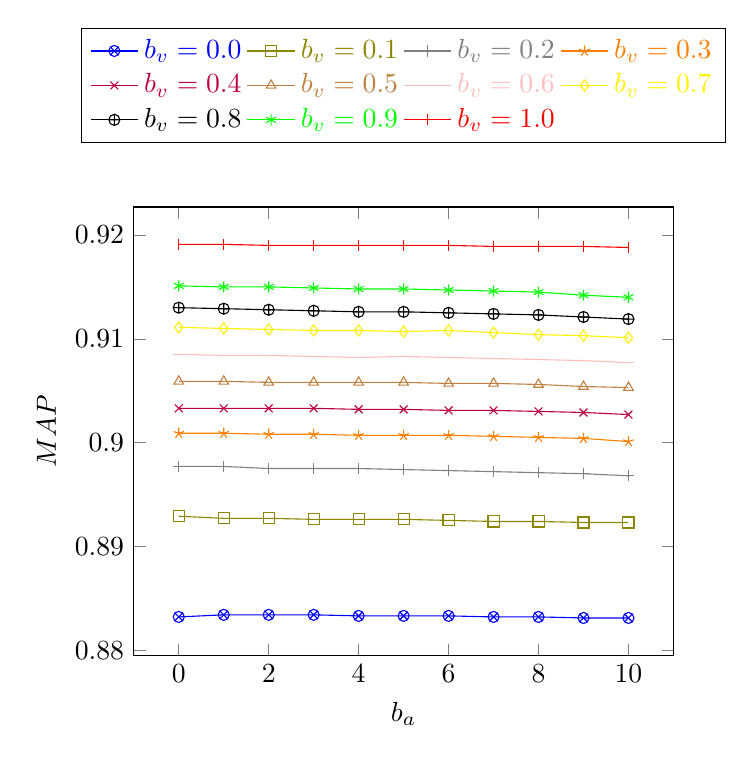
\begin{tikzpicture}
       \begin{axis}[
         xlabel=$b_a$,
         ylabel=$MAP$,
         legend style={at={(0.5, 1.4)}, anchor=north, legend columns=4},
         legend entries={
           [blue]$b_v = 0.0$,
           [olive]$b_v = 0.1$,
           [gray]$b_v = 0.2$,
           [orange]$b_v = 0.3$,
           [purple]$b_v = 0.4$,
           [brown]$b_v = 0.5$,
           [pink]$b_v = 0.6$,
           [yellow]$b_v = 0.7$,
           [black]$b_v = 0.8$,
           [green]$b_v = 0.9$,
           [red]$b_v = 1.0$
         }
       ]
           \addplot[mark=otimes, style=solid, color=blue] coordinates { (0, 0.8832) (1, 0.8834) (2, 0.8834) (3, 0.8834) (4, 0.8833) (5, 0.8833) (6, 0.8833) (7, 0.8832) (8, 0.8832) (9, 0.8831) (10, 0.8831) };
           \addplot[mark=square, style=solid, color=olive] coordinates { (0, 0.8929) (1, 0.8927) (2, 0.8927) (3, 0.8926) (4, 0.8926) (5, 0.8926) (6, 0.8925) (7, 0.8924) (8, 0.8924) (9, 0.8923) (10, 0.8923) };
           \addplot[mark=+, style=solid, color=gray] coordinates { (0, 0.8977) (1, 0.8977) (2, 0.8975) (3, 0.8975) (4, 0.8975) (5, 0.8974) (6, 0.8973) (7, 0.8972) (8, 0.8971) (9, 0.8970) (10, 0.8968) };
           \addplot[mark=star, style=solid, color=orange] coordinates { (0, 0.9009) (1, 0.9009) (2, 0.9008) (3, 0.9008) (4, 0.9007) (5, 0.9007) (6, 0.9007) (7, 0.9006) (8, 0.9005) (9, 0.9004) (10, 0.9001) };
           \addplot[mark=x, style=solid, color=purple] coordinates { (0, 0.9033) (1, 0.9033) (2, 0.9033) (3, 0.9033) (4, 0.9032) (5, 0.9032) (6, 0.9031) (7, 0.9031) (8, 0.9030) (9, 0.9029) (10, 0.9027) };
           \addplot[mark=triangle, style=solid, color=brown] coordinates { (0, 0.9059) (1, 0.9059) (2, 0.9058) (3, 0.9058) (4, 0.9058) (5, 0.9058) (6, 0.9057) (7, 0.9057) (8, 0.9056) (9, 0.9054) (10, 0.9053) };
           \addplot[mark=-, style=solid, color=pink] coordinates { (0, 0.9085) (1, 0.9084) (2, 0.9084) (3, 0.9083) (4, 0.9082) (5, 0.9083) (6, 0.9082) (7, 0.9081) (8, 0.9080) (9, 0.9079) (10, 0.9077) };
           \addplot[mark=diamond, style=solid, color=yellow] coordinates { (0, 0.9111) (1, 0.9110) (2, 0.9109) (3, 0.9108) (4, 0.9108) (5, 0.9107) (6, 0.9108) (7, 0.9106) (8, 0.9104) (9, 0.9103) (10, 0.9101) };
           \addplot[mark=oplus, style=solid, color=black] coordinates { (0, 0.9130) (1, 0.9129) (2, 0.9128) (3, 0.9127) (4, 0.9126) (5, 0.9126) (6, 0.9125) (7, 0.9124) (8, 0.9123) (9, 0.9121) (10, 0.9119) };
           \addplot[mark=asterisk, style=solid, color=green] coordinates { (0, 0.9151) (1, 0.9150) (2, 0.9150) (3, 0.9149) (4, 0.9148) (5, 0.9148) (6, 0.9147) (7, 0.9146) (8, 0.9145) (9, 0.9142) (10, 0.9140) };
           \addplot[mark=|, style=solid, color=red] coordinates { (0, 0.9191) (1, 0.9191) (2, 0.9190) (3, 0.9190) (4, 0.9190) (5, 0.9190) (6, 0.9190) (7, 0.9189) (8, 0.9189) (9, 0.9189) (10, 0.9188) };
       \end{axis}
    \end{tikzpicture}
    }
    \caption{Average over simple graphs}
    \label{fig:summary-ranking-norm-simple}
  \end{subfigure}
  \quad
  \begin{subfigure}{.45\textwidth}
    \resizebox{\textwidth}{!}{
    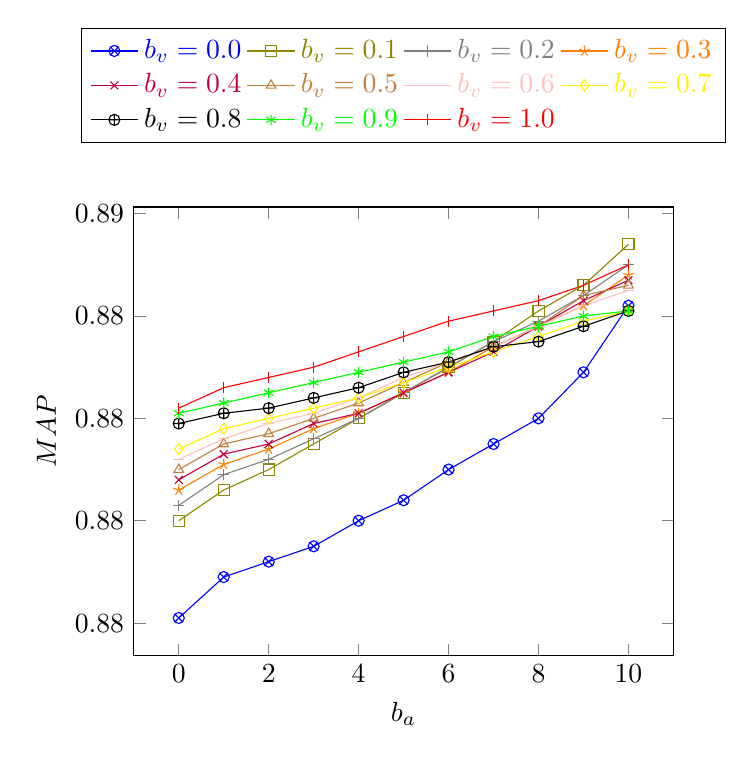
\begin{tikzpicture}
       \begin{axis}[
         xlabel=$b_a$,
         ylabel=$MAP$,
         legend style={at={(0.5, 1.4)}, anchor=north, legend columns=4},
         legend entries={
           [blue]$b_v = 0.0$,
           [olive]$b_v = 0.1$,
           [gray]$b_v = 0.2$,
           [orange]$b_v = 0.3$,
           [purple]$b_v = 0.4$,
           [brown]$b_v = 0.5$,
           [pink]$b_v = 0.6$,
           [yellow]$b_v = 0.7$,
           [black]$b_v = 0.8$,
           [green]$b_v = 0.9$,
           [red]$b_v = 1.0$
         }
       ]
           \addplot[mark=otimes, style=solid, color=blue] coordinates { (0, 0.8781) (1, 0.8789) (2, 0.8792) (3, 0.8795) (4, 0.8800) (5, 0.8804) (6, 0.8810) (7, 0.8815) (8, 0.8820) (9, 0.8829) (10, 0.8842) };
           \addplot[mark=square, style=solid, color=olive] coordinates { (0, 0.8800) (1, 0.8806) (2, 0.8810) (3, 0.8815) (4, 0.8820) (5, 0.8825) (6, 0.8830) (7, 0.8835) (8, 0.8841) (9, 0.8846) (10, 0.8854) };
           \addplot[mark=+, style=solid, color=gray] coordinates { (0, 0.8803) (1, 0.8809) (2, 0.8812) (3, 0.8816) (4, 0.8820) (5, 0.8825) (6, 0.8830) (7, 0.8835) (8, 0.8839) (9, 0.8844) (10, 0.8850) };
           \addplot[mark=star, style=solid, color=orange] coordinates { (0, 0.8806) (1, 0.8811) (2, 0.8814) (3, 0.8818) (4, 0.8821) (5, 0.8825) (6, 0.8829) (7, 0.8834) (8, 0.8838) (9, 0.8842) (10, 0.8848) };
           \addplot[mark=x, style=solid, color=purple] coordinates { (0, 0.8808) (1, 0.8813) (2, 0.8815) (3, 0.8819) (4, 0.8821) (5, 0.8825) (6, 0.8829) (7, 0.8833) (8, 0.8838) (9, 0.8843) (10, 0.8847) };
           \addplot[mark=triangle, style=solid, color=brown] coordinates { (0, 0.8810) (1, 0.8815) (2, 0.8817) (3, 0.8820) (4, 0.8823) (5, 0.8827) (6, 0.8831) (7, 0.8834) (8, 0.8838) (9, 0.8844) (10, 0.8846) };
           \addplot[mark=-, style=solid, color=pink] coordinates { (0, 0.8812) (1, 0.8816) (2, 0.8819) (3, 0.8821) (4, 0.8824) (5, 0.8828) (6, 0.8831) (7, 0.8834) (8, 0.8838) (9, 0.8842) (10, 0.8845) };
           \addplot[mark=diamond, style=solid, color=yellow] coordinates { (0, 0.8814) (1, 0.8818) (2, 0.8820) (3, 0.8822) (4, 0.8824) (5, 0.8827) (6, 0.8830) (7, 0.8833) (8, 0.8836) (9, 0.8839) (10, 0.8841) };
           \addplot[mark=oplus, style=solid, color=black] coordinates { (0, 0.8819) (1, 0.8821) (2, 0.8822) (3, 0.8824) (4, 0.8826) (5, 0.8829) (6, 0.8831) (7, 0.8834) (8, 0.8835) (9, 0.8838) (10, 0.8841) };
           \addplot[mark=asterisk, style=solid, color=green] coordinates { (0, 0.8821) (1, 0.8823) (2, 0.8825) (3, 0.8827) (4, 0.8829) (5, 0.8831) (6, 0.8833) (7, 0.8836) (8, 0.8838) (9, 0.8840) (10, 0.8841) };
           \addplot[mark=|, style=solid, color=red] coordinates { (0, 0.8822) (1, 0.8826) (2, 0.8828) (3, 0.8830) (4, 0.8833) (5, 0.8836) (6, 0.8839) (7, 0.8841) (8, 0.8843) (9, 0.8846) (10, 0.8850) };
       \end{axis}
    \end{tikzpicture}
    }
    \caption{Average over complex graphs}
    \label{fig:summary-ranking-norm-complex}
  \end{subfigure}
  \caption{MF normalisation parameters over simple and complex graphs}
  \label{fig:summary-ranking-norm}
\end{figure}


\subparagraph{Basic and MF-based approaches comparison.}

Given the outcome of the previous experiment, we set to $1.0$ the parameters of the Normalisations in the MF-based approach for the comparison between MF-based and basic ranking approaches of the graph summary.\\

Table~\ref{tab:summary-ranking-cmp} reports the MAP values of the basic and MF-based approaches over the Types summary of Dbpedia. We write the MAP value in bold for the approach that has the greatest. We observe that for a majority of the query complexities, the MF-based approach provides a better ranking than the basic approach.

This shows the benefits of the MF ranking model of normalising the data over two levels: the Normalisation~\ref{norm:content} allows to compare several solutions to a query regardless of different statistics they might have; with the Normalisation~\ref{norm:degree}, it is possible to rank solutions to a query that have different degree of a same attribute.

\begin{table}
	\centering
	\resizebox{.7\textwidth}{!}{
		\begin{tabular}{lc@{\hs}rr}
			\hline
			& \phantom{a} & Basic Approach & \gls{MF}-based Approach \\
			\cmidrule{3-4}
			1-1-4 & \phantom{a} & 0.8096 & \textbf{0.8102} \\
			1-1-3 & \phantom{a} & 0.8692 & \textbf{0.8698} \\
			1-1-2 & \phantom{a} & 1.0000 & 1.0000 \\
			3-4 & \phantom{a} & 1.0000 & 1.0000 \\
			2-2 & \phantom{a} & 0.7503 & \textbf{0.7870} \\
			1-5 & \phantom{a} & 0.9784 & \textbf{0.9791} \\
			1-4 & \phantom{a} & 0.8793 & \textbf{0.8867} \\
			1-3 & \phantom{a} & 0.6730 & \textbf{0.6744} \\
			1-2 & \phantom{a} & 0.8795 & \textbf{0.8977} \\
			1-1 & \phantom{a} & 0.9381 & \textbf{0.9447} \\
			10 & \phantom{a} & 0.9351 & \textbf{0.9439} \\
			9 & \phantom{a} & \textbf{0.9344} & 0.9433 \\
			6 & \phantom{a} & 0.7877 & \textbf{0.8699} \\
			5 & \phantom{a} & 0.8475 & \textbf{0.9111} \\
			4 & \phantom{a} & 0.8685 & \textbf{0.9089} \\
			3 & \phantom{a} & 0.8763 & \textbf{0.9154} \\
			2 & \phantom{a} & 0.9320 & \textbf{0.9389} \\
			\hline
		\end{tabular}
	}
	\caption[Comparison of the basic and MF-based ranking approaches on the \gls{typessummary} of DBpedia 3.3]{Comparison of the basic and \gls{MF}-based ranking approaches on the \gls{typessummary} of DBpedia 3.3}
	\label{tab:summary-ranking-cmp}
\end{table}


%\begin{figure}
	%\centering
	%\resizebox{.7\textwidth}{!}{
		%\begin{tikzpicture}
		%\begin{axis}[
			%compat=newest,
			%ymajorgrids,
			%ybar,
			%symbolic x coords={$1-1-4$,$1-1-3$,$1-1-2$,$3-4$,$2-2$,$1-5$,$1-4$,$1-3$,$1-2$,$1-1$,$10$,$9$,$6$,$5$,$4$,$3$,$2$},
			%enlargelimits=0.15,
			%ylabel={MAP},
			%x=2cm,
			%bar width=0.3cm,
			%xtick=data,
			%legend style={at={(0.5,-0.15)},
				%anchor=north,legend columns=-1},
		%]
		%\addplot coordinates {
			%($1-1-4$, 0.8096)
			%($1-1-3$, 0.8692)
			%($1-1-2$, 1.0000)
			%($3-4$,   1.0000)
			%($2-2$,   0.7503)
			%($1-5$,   0.9784)
			%($1-4$,   0.8793)
			%($1-3$,   0.6730)
			%($1-2$,   0.8795)
			%($1-1$,   0.9381)
			%($10$,    0.9351)
			%($9$,     0.9344)
			%($6$,     0.7877)
			%($5$,     0.8475)
			%($4$,     0.8685)
			%($3$,     0.8763)
			%($2$,     0.9320)
		%};

		%\addplot coordinates {
			%($1-1-4$, 0.8102)
			%($1-1-3$, 0.8698)
			%($1-1-2$, 1.0000)
			%($3-4$,   1.0000)
			%($2-2$,   0.7870)
			%($1-5$,   0.9791)
			%($1-4$,   0.8867)
			%($1-3$,   0.6744)
			%($1-2$,   0.8977)
			%($1-1$,   0.9447)
			%($10$,    0.9439)
			%($9$,     0.9433)
			%($6$,     0.8699)
			%($5$,     0.9111)
			%($4$,     0.9089)
			%($3$,     0.9154)
			%($2$,     0.9389)
		%};

		%\legend{Basic,MF-based}
		%\end{axis}
		%\end{tikzpicture}
	%}
	%\caption{Comparison of the basic and MF-based ranking approaches on the Types summary of DBpedia 3.3}
%\end{figure}

